\documentclass{book}

\usepackage[utf8x]{inputenc}
\usepackage{url}
\usepackage{hyperref}
\usepackage{enumerate}
\usepackage{adjustbox}
\usepackage{graphicx}
\usepackage{amssymb}
\usepackage{bussproofs}
\usepackage{amsthm}
\usepackage[portuguese]{babel}

\usepackage{color}
\definecolor{keywordcolor}{rgb}{0.7, 0.1, 0.1}   % red
\definecolor{commentcolor}{rgb}{0.4, 0.4, 0.4}   % grey
\definecolor{symbolcolor}{rgb}{0.0, 0.1, 0.6}    % blue
\definecolor{sortcolor}{rgb}{0.1, 0.5, 0.1}      % green

\usepackage{listings}
\def\lstlanguagefiles{lstlean.tex}
\lstset{language=lean}


\begin{document}

\title{Matemática Discreta em Lean}
\author{many}

\maketitle
\tableofcontents

\chapter{Introdução}
A linguagem matemática é, atualmente, caracterizada por seu rigor formal, e possibilidade de abstração sobre diferentes contextos. Somos capazes de descrever e avaliar situações impensáveis mesmo externas a realidade paupável, e obter respostas para problemas que seriam impossíveis sem o uso desse rigor. De fato, o surgimento da matemática formal é frequentemente creditado a Grécia, sec. VI a.c., embora haja registros retratando uso de conhecimento matemático no Egito muito antes disso. Tal fato é justificado uma vez que apenas na Grécia surge o questionamento de \textit{como sabemos} e não apenas \textit{o que sabemos}. A partir daí, as bases para desenvolver um conhecimento sólido poderiam ser iniciadas, partindo da filosofia ao método científico e formalismo matemático.

%Pensar em uma forma deu juntar as duas partes sem perder informação

Existem evidências do uso da matemática já por volta de 3000 a.c, onde povos antigos como os mesopotâmicos, egípcios e moradores de Ebla utilizavam a aritimética, álgebra e a geometria para taxação, comércio, trocas, astronomia e na formulação de calendários e marcação do tempo corrente. 

Os registros matemáticos (em texto) mais antigos vem da Mesopotâmia e do Egíto, e são datados aproximadamente entre 2000 a.c e 1800 a.c, mas muitos estudiosos consideram a Grécia Antiga como o berço da matemática, onde, por volta de 600 a.c, os Pitagóricos iniciaram o estudo da matemática como uma "disciplina demonstrativa" e introduziram o raciocínio dedutivo e o rigor matemático em provas formais.

%Colocar segunda parte histórica?

Aqui, a lógica entra exatamente para questionar \textit{como sabemos}, ou melhor, como podemos ter certeza de que concluimos coisas acertadas partindo de um contexto inicial. A formalização do processo de raciocínio garante que \textit{construimos um castelo de cartas adicionando cola as partes}.

Não devemos, no entanto, nos limitar a discutir lógica como ferramenta relacionada a teoremas ou metafísica. Esse ramo é presente no estudo da linguagem (lógica informal), processos industriais e computação (métodos formais), por exemplo. %Pesquisadores imaginavam que, quando fossem capazes de descrever o pensamento humano em termos lógicos, seriam tambem capazes de produzir uma máquina inteligente.

\section{Lógica formal e linguagem natural}
% uma referencia interssante
% http://www.pucrs.br/edipucrs/online/pesquisa/pesquisa/artigo11.html
A linguagem humana é conhecidamente um emaranhado gigantesco de simbolos, gestos, palavras, sentidos, interpretações. Essa é fruto de lapidação através de milênios, do que se iniciou com uma linguagem básica animalesca, chegando a complexidade atual em um processo evolutivo constante; assim ocorreu com a fala e escrita.

É impossível afirmar, portanto, que uma língua, digamos o português, é ineficiente na transmissão de significados, sendo fruto de evolução pura e constante. De fato, os linguistas se dedicam em grande parte a desvendar os mecanismos segundo os quais a lingua se molda e se torna tão eficiente, transmitindo significados profundos, dificeis até mesmo de serem explicados formalmente. Tal língua capta noções como: medo; incerteza; possibilidade; instinto, etc. naturalmente imprecisas.

Em contraparte, a linguagem lógica busca firmar o processo de pensamento sob regras bem definidas, que às vezes não captam as noções da linguagem natural em sua completude, no entanto, permitem discutir assertivas que seriam contraintuitivas para um ouvinte desinformado. Por exemplo, podemos afirmar que \textit{toda vaca voadora come gente}, e isso não fará o menor sentido a não ser que estabeleçamos essa como uma afirmativa lógica. Esse é um exemplo caricato que esclarece como a lógica nos permite discutir conclusões acertadas, que seriam pouca acessíveis apenas utilizando de um arcabouço de linguagem natural.

[Acho que aqui podemos introduzir para discutir um problema de lógica usando linguagem natural. Mostrar como ficaria extensivo e pouco claro "Procure argumentar uma solução para o problema: "]

Mais uma vez, é importante reforçar que a linguagem natural é um meio extremamente eficiente de transmissão de significaos. Há um ramo da lógica chamado lógica informal que lida com o modo como expressamos o raciocínio através da lingua: argumentação e falácias, por exemplo. É possível discutir se \textit{Um ser humano sem linguagem enlouqueceria}.

\section{Sobre Sistemas Dedutivos}
% Um pouco sobre sistemas, DN, Cálculo de Sequentes e Resolução, pex.
Para motivação, considere o seguinte problema: \textit{Você acorda em uma sala com duas portas. Uma dá para a liberdade, e a outra leva a morte, mas você não sabe qual é cada uma. Junto a cada porta há um guarda. Um dos guardas é sempre sincero, enquanto o outro é sempre mentirozo. Você tem direito a uma única pergunta para decidir qual porta tomar. O que você faz?}

Esse é claramente um problema envolvendo um raciocínio complexo, e, se tratando da sua vida em jogo, exige plena certeza da solução antes de uma resposta definitiva. De fato, seremos capazes de formalizar problemas desse tipo, e obter métodos de derivação para obter um prova para a resposta.

\section{Provadores, ATP e ITP}
Como computadores tem sido usados no processo de provas desse tipo.

\chapter{Introdução ao LEAN}
Capítulo sobre o provador utilizado no curso: o LEAN

\section{Teoria dos tipos}
Descrição superficial do teoria dos tipos para justificar o pardigma PAT.
Tambem justifica como o LEAN provas as coisas.

\section{Provas usando LEAN}
Exemplos (avancados) de provas utilizado LEAN.

\chapter{Introdução ao Lean }
% https://leanprover.github.io/theorem_proving_in_lean/introduction.html

Ao final do último capítulo, definimos duas classes fundamentais de ferramentas de auxílio a prova de teoremas, os \textit{ATPs} e \textit{ITPs}.
Esses grupos de ferramentas em geral são muito bem definidos, e distanciados, mantendo um espaço vazio entre si, o que pode parecer desvantajoso:o  matemático pode desejar algo entre a prova automática e interativa, ou o acesso a ambos os recursos numa mesma ferramenta.

O provador de teoremas Lean\footnote{documentação, ambiente e tutoriais estão disponiveis em: leanprover.github.io} busca preencher essa lacuna: uma única ferramenta contendo o melhor de ambos os mundos acessíveis.
Nesse sentido, age como uma \textit{ponte entre os dois mundos}.

O ambiente do Lean suporta interação, construção de termos, e verificação passo-a-passo das expressões desenvolvidas.
Lean implementa o chamado \textit{calculus of constructions}, ou cálculo de contruções, um sistema dedutivo bastante poderoso, que contém os demais sistemas a serem discutidos ao longo do livro, tais como Lógica de Proposições, ou Lógica de Primeira Ordem.

Um usuário inicial pode se deparar com algumas dúvidas pertinentes: \textit{porque contruir um termo é uma prova?}, \textit{consigo desenvolver provas top-down e botton-up?}, ou \textit{como conhecer as bibliotecas que o Lean já tem implementadas?}Algumas dessas dúvidas são esclarecidas logo mais, enquanto outras serão deixadas para pŕatica ao longo dos proximos capítulos.

\section{Teoria dos tipos}
% https://leanprover.github.io/theorem_proving_in_lean/dependent_type_theory.html
% https://en.wikipedia.org/wiki/Type_theory
\textit{Teoria dos Tipos} é uma classe de linguagens poderosa, que permite desenvolver assertivas bem definidas sobre definições matemáticas, ou exprimir conceitos desde os abstratos aos mais paupáveis.
De fato, essa é uma linguagem bastante expressiva, e útil para definição de elementos formais; até certo ponto, é semelhante a noção de teoria dos conjuntos.

No entanto, em muitos contextos, é razoável utilizar uma linguagem com ferramental teórico capaz de lidar com uma gama de elementos distitos, pertencentes a diversas classes, \textit{tipos distintos}.
Isso ocorre frequentemente quando tratamos de objetos matemáticos, e formalismos nesse sentido: o elemento $1$ pode ter o tipo natural ou real, assim como $[1,2,3, ...]$ pode expressar o tipo de uma lista de inteiros, dependendo da interpretação e contexto dados.
Claramente lidamos constantemente com elementos de tipos distintos, objetos que se relacionam, e tipos que se relacionam.
Pra isso, \textit{teoria dos tipos} se mostra extremamante útil.

Lean, em especial, implementa uma versão da linguagem chamada \textit{Calculo das Construções}, ou \textit{Calculus of Constructions}. A partir dos próximos exemplos, o leitor é convidado a acompanhar fazendo a intelação da ferramenta, ou através do \textit{Lean Web Editor\footnote{leanprover.github.io/live/latest/}}.

\subsection{Noções Fundamentais}
Em teoria dos tipos, tudo tem um tipo definido. Essa é uma exigência razoável; de fato, somos capazes de \textit{tipar} qualquer elemento dentro de um contexto definido, em uma linguagem adequada. Vejamos alguns exemplos em Lean:

\vspace{5mm}
\begin{lstlisting}
    -- abaixo declaramos algumas variaveis e usamos o
    -- comando #check para checar o tipo do elemento
    variable b : bool
    variable n : ℕ
    variable f : ℕ → ℕ
    variable g : ℕ × ℕ → ℕ

    #check b            -- b : bool
    #check 1            -- 1 : ℕ
    #check n + 1        -- n + 1 : ℕ

    #check f n          -- f n : ℕ
    #check g (1,n)      -- g (1, n) : ℕ
\end{lstlisting}
\vspace{5mm}

\noindent O comando \textit{variable} declara uma nova variável no contexto.
A partir disso, somos capazes de checar os tipo.

Note nas linhas $5$ e $6$ que $f$ e $g$ podem ser interpretadas como funções de naturais em naturais, então pudemos fazer a aplicação em $12$ e $13$, recebendo $f n$ e $g (1,n)$ como naturais.
Essa saída faz sentido em termos de tipo: sabemos que a aplicação tem tipo natural, embora não saibamos \textit{qual} natural.

Um leitor curioso pode questionar \textit{se tudo tem um tipo, qual tipo dos tipos?} ou ainda ir além, e \textit{qual o tipo do tipo dos tipos?} E essas perguntas podem ser respondidas novamente através do Lean:

\vspace{5mm}
\begin{lstlisting}
    #check ℕ            -- ℕ : Type
    #check bool         -- bool : Type

    -- considere Type = Type 0
    #check Type 0       -- Type : Type 1
    #check Type 1       -- Type : Type 2
    #check Type 2       -- Type : Type 3
\end{lstlisting}
\vspace{5mm}

\noindent Essa pode ser uma resposta \textit{frustrante} ou \textit{brilhante}.
Os tipos básicos em Lean tem o tipo \textit{Type}, ou \textit{Type 0}, enquanto o proprio tipo \textit{Type 0} tem tipo \textit{Type 1} quem tem tipo \textit{Type 2} e assim por diante.

Essa noção de hierarquia de tipos é uma solução proposta inicialmente por Russel, e posteriormente desenvolvida por Chwistek e Ramsey, em sua \textit{teoria simples dos tipos}, para evitar o conflito entre a teoria dos conjuntos de Frege, e o paradoxo de Russel.
De forma simples, a hierarquia de tipos evita o autorreferenciamento, em que um elemento tem o próprio tipo.

O que o Lean se propõe a fazer, portanto, é oferencer um ambiente para tratar da álgebra de tipos, implementando conceitos como \textit{abstração} e \textit{aplicação}, ou \textit{tipos dependentes}.

\subsection{Proposições como Tipos}
% leanprover.github.io/theorem_proving_in_lean/propositions_and_proofs.html
Entramos em uma das discussões mais fundamentais sobre o \textit{como Lean provas um teorema}, e para isso, introduzimos a noção de \textit{Proposições como Tipos}, através do tipo \textit{Prop}.

Considere um tipo \textit{Prop} cujos habitantes (elementos daquele tipo) representam uma \textit{prova daquela proposição}.
Em outras palavras, dada uma proposição que se deseje provar, basta construirmos um termo \textit{habitante daquela proposição} através de aplicações, abstrações ou outras ténicas formais para lidar com os tipos.
Vejamoas um exemplo:

\vspace{5mm}
\begin{lstlisting}
    variables A B : Prop    -- A e B sao proposicoes

    variable h1 : A         -- h1 uma prova para A
    variable h2 : A → B     -- h2 uma prova para A → B

    example : B := h2 h1    -- h2 h1 prova para B
    #check h2 h1            -- h2 h1 : B
\end{lstlisting}
\vspace{5mm}

Acima, introduzimos sem maiores explicações algumas noções profundas sobre Lean, e lógica proposicional, que serão discutidas nos próximos capítulos.
No entanto, note que no contexto dado, fomos capazes de construir um termo \textit{h2 h1} que tem tipo \textit{B}, então costruimos uma prova para \textit{B}, na linha $6$; ainda podemos checar se esse termo tem o tipo desejado, em $7$.

Observe ainda, na linha $4$, em que criamos um elemento do tipo $A → B$, que anteriormente citamos como a noção de uma função que leva tipo $A$ em um tipo $B$.
Aqui, essa noção será extendida para a de \textit{implicação lógica}, tambem discutida no capítulo sobre lógica proposicional.

\section{Provas usando LEAN}
\begin{itemize}
    \item Exemplos (avancados) de provas utilizado LEAN.
    \item Podemos falar sobre o que é o tal "example" do item anterior.
    \item Talvez tambem falar sobre "theorem", e "lemma".
    \item Acho que "sections e namespaçes", não.
\end{itemize}

\subsection{Modo Termo}
Apresentação e exemplos

\subsection{Modo Tática}
Apresentação e exemplos

\subsection{Modo Cálculo}
Apresentação e exemplos

% será que faz sentido falarmos em aspectos praticos sobreo Lean, como onde ele está disponivel online, ou como conhecer os teormas basicos dispoiveis...

\chapter{Lógica Proposicional}
\section{Introdução}

\section{Regras de Inferência}
Quando nos comunicamos, é habitual utilizar diferentes estruturas de linguagem que nos aproximem do sentido que queremos dar a alguma sentença. Na lógica proposicional, esses padrões são também amplamente utilizados e importantes para a construção de fórmulas e serão melhor aprofundados a seguir.
%Sugestões
%Acho que poderíamos juntar a parte de semântica do capítulo 6 
%(na qual ele discute o que é algo ser verdadeiro ou falso e introduz as tabelas verdade) 
%com os capítulos anteriores (caps 2-5), 
%onde ele introduz as regras de inferência, a dedução natural e o Lean. 
%Então introduziríamos as regras, mostrando o seu equivalente na tabela verdade e também no Lean. 
%Depois dessa seção mostraríamos as árvores mais complexas de dedução natural tb dessa forma. 

\subsection{Implicação} 
A implicação é essencial para o condicionamento de sentenças. Se na lingua falada utilizamos a estrutura "Se ... então" para nos referirmos a acontecimentos que dependem de outros, na logica a ideia é muito semelhante.

Retornando aos primeiros problemas do capítulo, relembramos um dos problemas descritos:
\begin{center}
\textbf{Se Ana viajar para o Chile, conhecerá o Atacama}

\textbf{Se a família real não tivesse vindo ao Brasil, então o território se desintegraria}
\end{center}

Apesar das duas sentenças terem a mesma estrutura "Se... então", podemos perceber que as duas tem suas diferenças. Em particular, chamamos a segunda proposição de implicação contrafactual, pois ela afirma como o mundo possivelmente seria, caso a realidade fosse diferentes do que ela realmente é. Esse assunto é discutido por filósofos há seculos e Spinoza e Saul Kripke são nomes de destaque nesses estudos. Entretanto, a lógica matemática se debruça mais especialmente na primeira sentença.

Dessa forma, tomando a primeira sentença como objeto de estudo, como podemos valorar essa implicação?
Para começar a analisar a valoração dessa implicação pensemos em A correspondendo o evento "Ana viaja para o Chile" e B ao evento "Ana irá conhecer o Atacama". Temos, então, dois casos e uma tabela verdade correpondente:

\begin{center}

Caso 1: Ana viaja para o Chile 

Caso 2: Ana não viaja para o Chile

\end{center}

\begin{table}[htb]
\centering
\begin{tabular}{|l|l|l|}
\hline

\textbf{A} & \textbf{B} & \textbf{A $\to$ B} \\ \hline
V          & V          & V                  \\ \hline
V          & F          & F                  \\ \hline
F          & V          & V                  \\ \hline
F          & F          & V                  \\ \hline

\end{tabular}
\end{table}

No primeiro caso, Ana viaja para o Chile e A é verdadeiro. Dessa forma, para a implicação ser verdadeira, B precisa ver também verdadeiro.

No segundo caso, Ana não viaja para o Chile e A é falso.
Dessa forma, nada podemos dizer sobre o evento B e qualquer valor atribuído a ele torna a implicação verdadeira. A esse tipo de afirmação, chamamos de \textbf{verdadeira por vacuidade}.

A implicação é protagonista da regra chamada "regra da exclusão da implicação" ou \textit{Modus Ponens}("A maneira que afirma afirmando" ), ou seja:

\begin{center}

Se Ana viajar para o Chile, conhecerá o Atacama

Ana viajou para o Chile

Ana conheceu o Atacama

\end{center}

Escrito em dedução natural como:

\begin{prooftree}
    \AxiomC{$A \rightarrow B$}
    \AxiomC{A}
    \BinaryInfC{B}
\end{prooftree}

E com seu correspondente no Lean, sendo:

\vspace{5mm}
\begin{lstlisting} 

section
variable h1 : A → B
variable h2 : A

example : B := h1 h2
end

\end{lstlisting}
\vspace{5mm}

Por outro lado, existe também a "regra de inclusão da implicação". Uma vez que temos uma variável A e conseguimos derivar uma variável B, dizemos que \textbf{A implica em B}. E utilizamos em nossas árvores de dedução natural de tal forma:

\begin{prooftree}
    \AxiomC{$A$}
    \noLine
    \UnaryInfC{$\vdots$}
    \noLine
    \UnaryInfC{$B$}
    \UnaryInfC{$A \rightarrow B$}
\end{prooftree}

Enquanto no Lean:

\vspace{5mm}
\begin{lstlisting} 

example : A → B :=
assume h : A,
show B, from sorry

\end{lstlisting}
\vspace{5mm}

\subsection{Se e somente se}
%Vitoria

\subsection{Conjunção}
A regra da conjunção se refere ao uso ``e'' na linguagem informal, de forma que juntamos duas informações. Podemos ter frases como:
\begin{center}
\textbf{Santiago é a capital do Chile e o deserto do Atacama está localizado no Chile.}
\end{center}

Ao mesmo tempo, podemos utilizar o ``e'' para conectar duas informações que nem mesmo possuem relação entre si. Por exemplo, podemos dizer que:
\begin{center}
\textbf{Santiago é a capital do Chile e Bolsonaro é o presidente do Brasil.}
\end{center}
Quando utilizamos o ``e'', representado pelo símbolo $\land$ na lógica, o que de fato importa é estarmos unindo duas informações que são verdadeiras. Isso fica claro na tabela verdade abaixo, na qual é possível ver que quando $A$ ou quando $B$ são falsos, $A\land B$ é falso:

\begin{table}[htb]
\centering
\begin{tabular}{|l|l|l|}
\hline
\textbf{A} & \textbf{B} & \textbf{A $\land$ B} \\ \hline
V          & V          & V                  \\ \hline
V          & F          & F                  \\ \hline
F          & V          & F                  \\ \hline
F          & F          & F                  \\ \hline
\end{tabular}
\end{table}

Dessa forma, na dedução natural, podemos introduzir um ``e'', quando temos $A$ e também temos $B$. Assim, se $A$ e $B$ forem verdadeiros, $A \land B$ também vai ser. 

 \begin{prooftree}
     \AxiomC{A}
     \AxiomC{B}
     \BinaryInfC{$A \land B$}
\end{prooftree}

No Lean, representamos essa operação pela função $and.intro$, conforme o exemplo abaixo:
\vspace{5mm}
\begin{lstlisting} 
variables A B : Prop

example (h1 : A) (h2 : B) : A ∧ B :=
and.intro h1 h2
\end{lstlisting}
\vspace{5mm}

Seguindo esse raciocínio, é possível observar que sempre que temos $A \land B$, teremos $A$ e $B$ separadamente. Essa é a operação chamada de exclusão do ``e''.

Para excluir o $B$ de, por exemplo, $A \land B$, temos a chamada exclusão pela esquerda, conforme descrita abaixo:

 \begin{prooftree}
     \AxiomC{$A \land B$}
     \UnaryInfC{A}
\end{prooftree}

No Lean, essa operação pode ser feita utilizando a função $and.left$, conforme o código a seguir: 
\vspace{5mm}
\begin{lstlisting} 
variables A B : Prop

example (h1 : A ∧ B): A :=
and.left h1
\end{lstlisting}
\vspace{5mm}

Alternativamente, é possível realizar a mesma operação da seguinte forma:
\vspace{5mm}
\begin{lstlisting} 
variables A B : Prop

example (h1 : A ∧ B): A :=
h1.left
\end{lstlisting}
\vspace{5mm}
Para excluir o $A$, temos a chamada exclusão pela direita:

 \begin{prooftree}
     \AxiomC{$A \land B$}
     \UnaryInfC{B}
\end{prooftree}

No Lean, essa operação é realizada utilizando a função $and.right$, de maneira semelhante ao que foi descrito anteriormente para o $and.left$. 

\subsection{Disjunção}

A regra da disjunção se refere ao uso do ``ou''. Na linguagem informal, podemos utilizá-lo para expressar situações excludentes, como da seguinte forma:
\begin{center}
\textbf{Alexandre vai viajar para o Atacama ou Alexandre vai viajar para Santiago.}\\
\end{center}
Nesse caso, é possível que uma pessoa compreenda que somente uma das duas situações vai ocorrer, ou seja, que Alexandre somente vai para um dos dois lugares no Chile. Contudo, quando utilizamos o  ``ou'' na lógica, representado pelo símbolo $\lor$, também estamos levando em consideração situações nas quais ambas as proposições são verdadeiras. Dessa forma, conforme indicado na tabela verdade a seguir, a sentença formada pelo ``ou'' será verdadeira quando somente $A$ for verdadeiro, quando somente $B$ for verdadeiro ou quando ambos forem verdadeiros. 

\begin{table}[htb]
\centering
\begin{tabular}{|l|l|l|}
\hline
\textbf{A} & \textbf{B} & \textbf{A $\lor$ B} \\ \hline
V          & V          & V                 \\ \hline
V          & F          & V                 \\ \hline
F          & V          & V                 \\ \hline
F          & F          & F                 \\ \hline
\end{tabular}
\end{table}

Não só o ``ou'' formará uma sentença verdadeira quando uma ou ambas as situações forem verdadeiras, como também quando ambas as situações forem verdadeiras, mas não possuírem nenhuma relação entre si. Por exemplo, a seguinte sentença é verdadeira: 
\begin{center}
\textbf{Santiago é a capital do Chile ou Bolsonaro é o presidente do Brasil.}\\
\end{center}

É verdadeiro que Santiago é a capital do Chile e que Bolsonaro é o presidente do Brasil. Logo, toda a sentença é verdadeira, apesar de não soar de forma natural na linguagem informal.

Como o ``ou'' é verdadeiro mesmo que somente um de seus elementos seja verdadeiro, na dedução natural, é possível introduzir um ``ou'' tendo somente $A$ ou somente $B$. Logo, pode-se formar $A \lor B$ da seguinte forma:
\begin{prooftree}
     \AxiomC{A}
     \UnaryInfC{$A \lor B$}
\end{prooftree}

No Lean, essa operação de introdução do ``ou'' é realizada utilizando a função $or.inl$. Essa função indica que queremos adicionar o $A$ do lado esquerdo do $\lor$ (por isso, ``or include left''). Dessa forma, teremos o seguinte código: 
\begin{lstlisting} 
variables A B : Prop

example (h1 : A): A ∨ B :=
or.inl h1
\end{lstlisting} 

Alternativamente, é possível realizar a introdução do $\lor$ a partir do $B$:
\begin{prooftree}
     \AxiomC{B}
     \UnaryInfC{$A \lor B$}
\end{prooftree}

Nesse caso, como o $B$ está sendo adicionado à direita do $\lor$ utilizamos a função $or.inr$ no Lean (ou seja,  ``or include right''). 

\begin{lstlisting} 
variables A B : Prop

example (h1 : B): A ∨ B :=
or.inr h1
\end{lstlisting} 

Exclusão do ``ou'': 

\begin{prooftree}
    \AxiomC{$A \lor B$}
    \AxiomC{$A$}
    \noLine
    \UnaryInfC{$\vdots$}
    \noLine
    \UnaryInfC{$C$}
    \AxiomC{$B$}
    \noLine
    \UnaryInfC{$\vdots$}
    \noLine
    \UnaryInfC{$C$}
    \TrinaryInfC{$C$}
\end{prooftree}
     
Código Lean de exclusão do ``ou'':
\begin{lstlisting} 
variables A B C D : Prop

example (h1 : A → C) (h2 : B → C) (h3: A ∨ B): C :=
or.elim h3
(assume h4: A,
show C, from h1 h4)
(assume h4: B, 
show C, from h2 h4)
\end{lstlisting} 


\subsection{Negação}
%Incluir um exemplo de algum "quebra-cabeça"
A negação de $A$ é  representada  em  símbolos por $\neg A $. 
Mostrar que $\neg A $ ocorre, em termos lógicos, é o mesmo que mostrar que $A $ leva a uma contradição. Em dedução natural, temos uma prova que tem a seguinte árvore, na qual $\bot$ é o símbolo para falso, contradição ou absurdo:
\begin{prooftree}
    \AxiomC{A}
    \noLine
    \UnaryInfC{$\vdots$}
    \noLine
    \UnaryInfC{$\bot$}
    \UnaryInfC{$\neg A$}
\end{prooftree}

Começamos supondo $A$. Em seguida, continuamos a prova aplicando as regras  já apresentadas, representadas pelos três pontinhos na árvore de dedução natural, até chegarmos a uma contradição. 

A pergunta a se fazer em seguida é: de que forma uma contradição aparece numa prova, ou seja, como a encontramos? Suponha, por exemplo, que ao construir uma prova temos uma hipótese $A$ que nos leva a concluir que uma outra hipotése $B$ ocorre ao mesmo tempo que $\neg B$ também ocorre, no entanto se temos $B$ e  $ \neg B $, então temos uma contradição.
Em dedução natural, representamos essa ideia por:

%Completar a árvore incluindo A E \not A
\begin{prooftree}
    \AxiomC{$\neg B$}
    \AxiomC{B}
    \BinaryInfC{$\bot$}
\end{prooftree}

%Falar de false.elim e show false, from 

Uma vez apresentado o símbolo para \textit{falso}, a seguir apresentamos o símbolo para \textit{verdadeiro}. No entanto,  \textit{verdadeiro} ou \textit{true} não possui regra de eliminação, apenas a regra de introdução:

%Árvore da regra de introdução do true

No lean, obtemos $\neg A$ com o comando \verb| \not A|.
\subsection{Prova por contradição}
Existe um estilo de fazer matemático conhecido como "matemática construtivista" que nega a equivalência de $\neg \neg A$ e $ A$. Uma prova de que algo é verdadeiro deveria fornecer evidências explícitas de que uma declaração é falsa, em vez de evidências de que ela não pode ser falsa. 

Antes de utilizar a prova por absurdo precisamos abrir o modo clássico do lLean.

\section{Dedução Natural}

\section{Exercícios}

\newenvironment{bprooftree}
{\leavevmode\hbox\bgroup}
{\DisplayProof\egroup}
  
\chapter{Lógica de Primeira Ordem}
    
    Até agora, vimos Lógica Proposicional, em que variáveis proposicionais podem ser valoradas como verdadeiras ou falsas. Esse sistema lógico, porém, contém limitações. Considere, por exemplo, a afirmação de que todo natural é maior do que ou igual a zero.
    Ou a afirmação de que existe número natural que é primo e é par. Como representar isso em Lógica Propocional? Precisamos de um sistema lógico que saiba lidar com objetos e suas propriedades e relações.

    Talvez esses exemplos não tenham demonstrado a necessidade de tal sistema lógico. Porém, acredite: ao final deste capítulo, essa necessidade ficará evidente.

    \section{Sintaxe}

    A sintaxe de um sistema lógico aborda basicamente os símbolos que são utilizados para representá-lo. Portanto, nesta seção, serão abordados funções, predicados, relações e quantificadores, dentre eles $\forall$ e $\exists$.

    \subsection{Funções, Predicados e Relações}

        Dentro de Lógica de Primeira Ordem, funções, predicados e relações são mapeamentos que, dado algum elemento do domínio, retornam uma proposição ou outro elemento do domínio. Parece confuso? Vamos olhar um exemplo.

        \begin{center}
            $x$ natural é par ou ímpar.            
        \end{center}

        Nosso domínio, neste caso, são os números naturais ($\mathbb{N}$). Dizemos que \textit{par} é ``algo"\space que recebe um número e retorna $V$ ou $F$. Chamamos isso de \textbf{predicado}. Sendo assim, podemos escrever:

        \begin{center}
            $par(x) \lor impar(x)$.
        \end{center}

        A partir deste exemplo, podemos extrair alguns símbolos para exemplificar a construção de um sistema lógico de primeira ordem.

        \begin{itemize}
            \item O domínio são os naturais;
            \item Os objetos são os números $0$, $1$, $2$ etc.;
            \item Existem \textbf{funções}, como \textit{adição} e \textit{subtração}, que recebem (zero ou mais) números e retornam outros números;
            \item Existem \textbf{predicados}, como \textit{par} e \textit{ímpar}, que recebem um número e retornam $V$ ou $F$;
            \item Existem \textbf{relações}, como \textit{igual} e \textit{menor}, que recebem dois números e retornam $V$ ou $F$.
        \end{itemize}

        Os objetos pertencentes ao domínio, chamados constantes, como o $1$ e o $4$, no exemplo, podem ser considerados funções que tomam zero elementos. Além disso, podemos considerar predicados que tomam zero elementos como os valores lógicos $\top$ e $\bot$.

        Expressões que representam elementos do domínio(incluindo funções de elementos) são chamados de \textbf{termos}. Alguns exemplos:

        \begin{itemize}
            \item $5$
            \item $sucessor(10)$ (função sucessora, retorna o elemento acrescido de $1$)
            \item $33+44$
        \end{itemize}

        Observe que o símbolo para a função de adição está ``infixo"; poderíamos ter representado como $+(33, 44)$ ou $adicao(33, 44)$.
        
        Expressões que retornam $V$ ou $F$ são chamadas \textbf{fórmulas}:

        \begin{itemize}
            \item $maiorDoQue(1,2)$ ($1 > 2$)
            \item $par(10) \lor impar(5)$
            \item $2=2$
        \end{itemize}

        O Lean é muito eficiente em expressar Lógica de Primeira Ordem. Vejamos nosso exemplo:

        \begin{lstlisting}
constant U : Type
constant zero : U
constant par : U → Prop
constant primo : U → Prop
constant igual : U → U → Prop
constant adicao : U → U → U
\end{lstlisting}

        Pelo fato de que o Lean é baseado em \textit{Teoria dos Tipos}, declaramos um novo tipo \lstinline{U}. Podemos intuitivamente considerá-lo como ``universo"\space ou ``domínio". Por exemplo, o conjunto dos naturais.

        Foi declarado um objeto chamado \lstinline{zero} do tipo \lstinline{U} (nossa analogia com o zero natural).
        \lstinline{par} é um predicado, pois toma um elemento do tipo \lstinline{U} e retona um elemento do tipo proposição (\lstinline{Prop}).

        \lstinline{adicao} é uma função que toma dois elementos do tipo \lstinline{U} e retorna outro do mesmo tipo. Ora, podemos constatar:

        \begin{lstlisting}
#check par zero
#check adicao zero zero
#check par (adicao zero zero)
\end{lstlisting}

        O \lstinline{#check} da linha $1$ informa que a expressão tem tipo \lstinline{Prop}; na linha $2$, tipo \lstinline{U}; e, na linha $3$, tipo \lstinline{Prop}. Importante observar o papel dos parênteses acima, para que \lstinline{par} receba apenas um elemento.

        Uma função (ou relação) que recebe mais de um elemento tem notação \lstinline{U → U → U}. A notação para predicados (\lstinline{U → Prop}) e relações (\lstinline{U → U → Prop}) funciona como se ambas fossem funções, porém retornassem \lstinline{Prop}. 

        Vários conjuntos estão nas bibliotecas padrão do Lean, como os naturais, utilizados nos exemplos anteriores. O comando para o símbolo \lstinline{ℕ} é \lstinline{\nat} ou \lstinline{\N}.

        \begin{lstlisting}
constant zero : ℕ
#check zero + zero
\end{lstlisting}

        O \lstinline{#check} da linha $2$ retorna algo do tipo \lstinline{ℕ}.

        Podemos misturar Lógica Proposicional com Lógica de Primeira Ordem:

        \begin{lstlisting}
constant U : Type
constant zero : U
constant par : U → Prop
constant primo : U → Prop
constant igual : U → U → Prop
constant adicao : U → U → U

#check ¬ (par zero ∨ par (adicao zero zero)) ∧ primo zero
\end{lstlisting}

        E o \lstinline{#check} nos retorna algo do tipo \lstinline{Prop}.

    \subsection{Quantificador Universal}

        Grande parte do poder da Lógica Proposicional se deve aos quantificadores.
        O símbolo $\forall$ é o quantificador universal, que representa ``para todo".
        Quando ele é seguido de uma variável e de uma expressão, ele indica que aquela expressão é verdadeira para toda variável do domínio.
        Por exemplo:

        \begin{itemize}
            \item $\forall x \ (par(x) \lor impar(x))$
            \item $\forall y \ (par(y) \rightarrow impar(y + 1))$
        \end{itemize}

        A primeira expressão nos diz que todo número é par ou ímpar (no caso dos naturais).
        A segunda diz que, para todo número, o fato dele ser par implica que seu sucessor é ímpar.
        
        No Lean, é possível obter o símbolo \lstinline{∀} digitando \lstinline{\all}. Os exemplos anteriores ficam assim:

        \begin{lstlisting}
constant U : Type
constant par : U → Prop
constant impar : U → Prop
constant sucessor : U → U

#check ∀ x : U, par x ∨ impar x
#check ∀ y : U, par y → impar (sucessor y)
\end{lstlisting}

        Os dois \lstinline{#check}'s nos retornam \lstinline{Prop}. Quando é utilizado o quantificador universal,
        por padrão devemos dizer o tipo da variável que o acompanha. No exemplo, \lstinline{x : U}. Porém, o Lean é
        esperto o suficiente pra inferir o tipo da variável sozinho, então na maioria dos casos não será um problema omiti-lo.

        Observe as três sentenças:

        \begin{itemize}
            \item $\forall x \ (par(x) \lor impar(x))$
            \item $\forall x \ par(x) \lor impar(x)$
            \item $\forall x \ (par(x)) \lor impar(x)$
        \end{itemize}

        Por uma questão de convenção, as duas últimas sentenças são equivalentes, enquanto a primeira é diferente.
        Neste contexto, estamos lidando com o \textbf{escopo} da variável $x$. A convenção diz, portanto, que o escopo da variável é o menor possível.
        
        Curiosamente, o modo como o Lean lida com escopo é diferente: \lstinline{∀ x : U, par x ∨ impar x} equivale a \lstinline{∀ x : U, (par x ∨ impar x)}.
        Ou seja, o Lean busca o maior escopo possível.

        Quando estamos lidando com quantificadores, a variável que o acompanha é dita \textbf{limitada} (\textit{bound}, em inglês).
        Na expressão $\forall x \ A(x)$, a variável $x$ é limitada.
        Isso significa que o $x$ não representa um valor em si, mas apenas um ``espaço reservado"\space para qualquer outra variável.
        Observe que a expressão $\forall y \ A(y)$ representa exatamente a mesma coisa.

        Uma variável que não é limitada é chamada \textbf{livre}. Por exemplo, considere a expressão $\forall x \ y \le x$.
        Ora, sabemos que $x$ representa uma ``espaço reservado"\space para toda variável do domínio. O que representa $y$, portanto?
        Um elemento específico do domínio. Digamos que o domínio é $\mathbb{N}$ e $y$ representa o elemento zero. Então a expressão é verdadeira.
        Sendo assim, se trocarmos $y$ por $z$ (que representa, neste caso, outro elemento), então não vale a expressão $\forall x \ z \le x$.
        Observe como trocar $y$ por $z$ fez toda a diferença!

        No exemplo anterior, tanto $y$ quanto $z$ são variáveis livres. Quando uma expressão \textbf{não} contém variáveis livres, é chamada sentença.

        Quantificadores também possuem regras de introdução e eliminação. Vejamos:
        
        \begin{center}
            \begin{bprooftree}
                \AxiomC{$A(y)$}
                \RightLabel{\scriptsize $\forall I$}
                \UnaryInfC{$\forall x \ A(x)$}
            \end{bprooftree}
            \begin{bprooftree}
                \AxiomC{$\forall x \ A(x)$}
                \RightLabel{\scriptsize $\forall E$}
                \UnaryInfC{$A(t)$} 
            \end{bprooftree}
        \end{center}

        A regra da esquerda demonstra a \textbf{introdução} do quantificador universal. Ela vale quando $y$ não é livre em nenhuma hipótese não cancelada.
        A intuição neste caso é que, dado que vale $A(y)$ para algum $y$ qualquer, então podemos dizer que vale para todo $y$. Mudamos o nome da variável apenas
        pra que a operação fique mais evidente e intuitiva.

        A regra da direita demonstra a \textbf{eliminação} do quantificador universal. A intuição, neste caso,
        é que, se $A(x)$ vale para todo $x$, então vale para algum $t$ qualquer do domínio.

        Observe a semelhança dessas regras com aquelas relativas à implicação. No caso da introdução da implicação, assumimos $A$ e provamos $B$, então $A \rightarrow B$.
        No caso da introdução do quantificador universal, assumimos $x$ e mostramos $A(x)$, então $\forall x \ A(x)$.
        Para a eliminação da implicação, temos $A \rightarrow B$ e $A$, então temos $B$. Já no caso da eliminação do quantificador, temos $\forall x \ A(x)$ e $y$, então $A(y)$.

        Vejamos um exemplo aplicando essas regras. Observe como derivar $\forall x \ A(x) \land B(x)$ a partir de $\forall x \ A(x)$ e $\forall x \ B(x)$:

        \begin{center}
            \begin{bprooftree}
                \AxiomC{$\forall x \ A(x)$}
                \RightLabel{\scriptsize $\forall E$}
                \UnaryInfC{$A(y)$}
                \AxiomC{$\forall x \ B(x)$}
                \RightLabel{\scriptsize $\forall E$}
                \UnaryInfC{$B(y)$}
                \RightLabel{\scriptsize $\land I$}
                \BinaryInfC{$A(y) \land B(y)$}
                \RightLabel{\scriptsize $\forall I  $}
                \UnaryInfC{$\forall x \ A(x) \land B(x)$}
            \end{bprooftree}
        \end{center}

        Ora, e como representar isso em Lean? Vejamos a introdução:

        \begin{lstlisting}
constant U : Type
constant A : U → Prop

example : ∀ x, A x :=
    assume y,
    show A y, from sorry
\end{lstlisting}

        Estamos mostrando $\forall x \ A(x)$ da seguinte forma: assumimos um $y$ qualquer e provamos $A(y)$.
Neste caso, necessitamos de uma prova de $A(y)$, o que justifica o uso do \lstinline{sorry}.

        Observe, agora, a regra da eliminação:

        \begin{lstlisting}
constant U : Type
constant A : U → Prop
constant h1 : ∀ x, A x
constant t : U

example : A t :=
    h1 t
\end{lstlisting}

        Dado que sabemos que $\forall x \ A(x)$ (por \lstinline{h1}), podemos ``aplicar"\space $t$ e obter $A(t)$.

        Vejamos agora nosso exemplo que deriva $\forall x \ A(x) \land B(x)$ a partir de $\forall x \ A(x)$ e $\forall x \ B(x)$:

        \begin{lstlisting}
constant U : Type
constants A B : U → Prop
constant h1 : ∀ x, A x
constant h2 : ∀ x, B x

example : ∀ x, A x ∧ B x :=
    assume y,
        have h3 : A y, from h1 y,
        have h4 : B y, from h2 y,
    show A y ∧ B y, from and.intro h3 h4
\end{lstlisting}

    \subsection{Quantificador Existencial}

        O quantificador existencial é representado pelo símbolo $\exists$ e representa ``existe algum".
        Seguido de uma variável e uma expressão, ele significa que existe algum elemento no domínio tal que a expressão seja verdadeira.
        Alguns exemplos para o domínio dos naturais:

        \begin{itemize}
            \item $\exists x \ x \times x = x$
            \item $\exists y \ y \le 0$
            \item $\forall x \ \exists y \ par(y) \land y > x$
        \end{itemize}

        Ora, as expressões significam:

        \begin{itemize}
            \item Existe número natural que é igual ao seu quadrado ($0$ e $1$)
            \item Existe número menor do que ou igual a zero (o próprio zero)
            \item Para todo natural, existe um número que é par e maior do que ele
        \end{itemize}

        Em Lean, pode-se inserir \lstinline{∃} digitando \lstinline{\ex}. Vejamos os exemplos:

        \begin{lstlisting}
constant U : Type
constant par : U → Prop
constant maiorDoQue : U → U → Prop

#check ∃ x, x * x = x
#check ∃ y, y ≤ 0
#check ∀ x, ∃ y, par y ∧ maiorDoQue y x
\end{lstlisting}

        Como no caso do quantificador universal, a variável que acompanha o quantificador é dita \textbf{limitada}. Por exemplo, $x$ em $\exists x \ A(x)$.
        Variáveis não limitadas são \textbf{livres}.

        Vejamos as regras de introdução e eliminação desse quantificador:
        
        \begin{center}
            \begin{bprooftree}
                \AxiomC{$A(t)$}
                \RightLabel{\scriptsize $\exists I$}
                \UnaryInfC{$\exists x \ A(x)$}
            \end{bprooftree}
            \begin{bprooftree}
                \AxiomC{$\exists x \ A(x)$}
                \AxiomC{}
                \UnaryInfC{$A(y)$}
                \alwaysNoLine
                \UnaryInfC{$\vdots$}
                \UnaryInfC{$B$}
                \alwaysSingleLine
                \RightLabel{\scriptsize $\exists E$}
                \BinaryInfC{$B$}
            \end{bprooftree}
        \end{center}

        A primeira regra é a \textbf{introdução} do quantificador existencial. A intuição que segue é a de que, para mostrar que existe $x$ tal que  $A(x)$, basta mostrar que, para algum $t$, vale $A(t)$.

        A segunda regra é a \textbf{eliminação} e vale quando $y$ não é livre em $B$ e em nenhuma hipótese não cancelada. É uma regra um pouco menos trivial de se entender. Vamos lá:
        
        \begin{itemize}
            \item Digo que existe algum $x$ para o qual vale $A(x)$;
            \item Sei que, independentemente do $y$ que eu escolher, de $A(y)$ é possível derivar $B$;
            \item Concluo que vale B.
        \end{itemize}

        Outra forma de se interpretar essa regra é a seguinte: sei que existe $x$ tal que vale $A(x)$. A única maneira de eu ter certeza de que vale $B$ é mostrando que, pra qualquer $y$, $A(y)$ implica em $B$.
        Tenho que assumir um $y$ qualquer, pois não sei para qual $y$ especificamente vale $A(y)$.

        Tecnicamente, o que estamos fazendo é: dado que vale $\exists x \ A(x)$ e vale $\forall y \ (A(y) \to B)$, concluímos $B$, desde que $B$ não contenha $y$ livre. Para algumas pessoas,
        a utilização do quantificador universal ($\forall$) pode ser muito conveniente. Porém, para outras, pode ser um pouco mais confuso.

        Assim como as regras do quantificador universal se assemelham às da implicação, as regras mostradas acima se assemelham àquelas da introdução e eliminação do operador lógico ou. Observe:

        \begin{itemize}
            \item Assim como de $A$ eu derivo $A \lor B$, de $A(t)$ derivo $\exists x \ A(x)$. O que estamos derivando diz que pelo menos um dos argumentos é válido ou existe.
            \item Para mostrar $C$ de $A \lor B$, assumo $A$ e mostro $C$ e depois assumo $B$ e mostro $C$. No caso do nosso quantificador, para saírmos de $\exists x \ A(x)$ e chegarmos em $B$, assumo qualquer valor de $y$ e mostro que de $A(y)$ chego em $B$.
            Nos dois casos, estamos verificando se, em todas as possibilidades, conseguimos concluir o que queremos.
        \end{itemize}

        Vejamos um exemplo que utiliza as duas regras, mostrando $(\exists x \ A(x)) \land (\exists x \ B(x))$ a partir de $\exists x \ (A(x) \land B(x))$:

        \begin{center}
            \begin{bprooftree}
                \AxiomC{$\exists x \ (A(x) \land B(x))$}
                \AxiomC{}
                \UnaryInfC{$A(y) \land B(y)$}
                \RightLabel{\scriptsize $\land E$}
                \UnaryInfC{$A(y)$}
                \RightLabel{\scriptsize $\exists I$}
                \UnaryInfC{$\exists x \ A(x)$}
                \AxiomC{}
                \UnaryInfC{$A(y) \land B(y)$}
                \RightLabel{\scriptsize $\land E$}
                \UnaryInfC{$B(y)$}
                \RightLabel{\scriptsize $\exists I$}
                \UnaryInfC{$\exists x \ B(x)$}
                \RightLabel{\scriptsize $\land I$}
                \BinaryInfC{$(\exists x \ A(x)) \land (\exists x \ B(x))$}
                \RightLabel{\scriptsize $\exists E$}
                \BinaryInfC{$(\exists x \ A(x)) \land (\exists x \ B(x))$}
            \end{bprooftree}
        \end{center}

        Essas regras também podem ser utilizadas em Lean. Vejamos a introdução:

        \begin{lstlisting}
constant U : Type
constant A : U → Prop
constant t : U
constant h1 : A t

example : ∃ x, A x :=
    exists.intro t h1
\end{lstlisting}

        Para a introdução do quantificador existencial, utilizamos \lstinline{exists.intro}, que requer dois argumentos:
        um termo e uma prova de que a expressão vale para esse termo. É o que está sendo feito no código acima. Na linha $4$, sabemos que vale $A(t)$. Passando $t$ e $A(t)$
        como argumentos para \lstinline{exists.intro}, temos $\exists x \ A(x)$.

        Vejamos a regra da eliminação:

        \begin{lstlisting}
constant U : Type
constant A : U → Prop
constant h1 : ∃ x, A x
constant B : Prop

example : B :=
    exists.elim h1
        (assume y (h2 : A y),
        show B, from sorry)
\end{lstlisting}

        Utilizamos \lstinline{exists.elim}, que toma dois argumentos: a expressão $\exists x \ A(x)$ e uma expressão que prova $B$ a partir de $y$ qualquer e $A(y)$.
        
        Observe como fica mais clara a consideração feita anteriormente com relação ao quantificador universal ($\forall$): estamos dando para \lstinline{exists.elim} as expressões $\exists x \ A(x)$ e $\forall y \ (A(y) \to B)$, e ela nos retorna $B$. Observe como o \lstinline{show} nos ajuda a mostrar isso:

        \begin{lstlisting}
example : B :=
    exists.elim h1
        (show ∀ y, A y → B, from
            assume y (h2 : A y),
            show B, from sorry)
\end{lstlisting}

        Vejamos nosso exemplo anterior, agora implementado em Lean, que mostra $(\exists x \ A(x)) \land (\exists x \ B(x))$ a partir de $\exists x \ (A(x) \land B(x))$:
        \begin{lstlisting}
constant U : Type
constants A B : U → Prop
constant h1 : ∃ x, A x ∧ B x

example : (∃ x, A x) ∧ (∃ y, B y) :=
    exists.elim h1
        (assume y (h2 : A y ∧ B y),
            have h3 : A y, from h2.left,
            have h4 : B y, from h2.right,
            have h5 : ∃ x, A x, from exists.intro y h3,
            have h6 : ∃ x, B x, from exists.intro y h4,
        show (∃ x, A x) ∧ (∃ y, B y), from and.intro h5 h6)
\end{lstlisting}
    \section{Semântica}
    
   A seção anterior abordou a sintaxe da lógica de primeira ordem, ou seja, apresentou os símbolos e estruturas das fórmulas deste sistema. A semântica, por outro lado, define a verdade das fórmulas pela \textbf{interpretação} e \textbf{valoração}.
    
    \subsection{Interpretações}
    
    \subsection{Verdade e modelos}
    
    \subsection{Exemplos}
    
    \subsection{Validação e consequência lógica}
    
    \subsection{Correção e completude}
    

    \section{Dedução Natural}
Como visto na seção anterior, devemos estabelecer as regras de inclusão e exclusão
de dedução para os quantificadores e para a igualdade. Listamos elas inicialmente:
\newline \textbf{Quantificador universal:}
 \newline 
 \begin{center}
 \begin{bprooftree}
    \AxiomC{$A(y)$}
    \RightLabel{\scriptsize $\forall I$}
    \UnaryInfC{$\forall x A(x)$}
\end{bprooftree}
\begin{bprooftree}
    \AxiomC{$\forall x A(x)$}
    \RightLabel{\scriptsize $\forall E$}
    \UnaryInfC{$A(t)$} 
\end{bprooftree}
\end{center}

Para inserir o quantificador universal devemos ter que a variável $y$ não deve estar 
atrelada em nenhuma hipótese, isto é, em todas as hipóteses não canceladasela não pode ser livre. 
\newline \textbf{Quantificador existencial:}

 \begin{center}
    \begin{bprooftree}
        \AxiomC{$A(t)$}
        \RightLabel{\scriptsize $\exists I$}
        \UnaryInfC{$\exists x A(x)$}
    \end{bprooftree}
    \begin{bprooftree}
        \AxiomC{$\exists x A(x)$}
        \AxiomC{}
        \UnaryInfC{$A(t)$}
        \alwaysNoLine
        \UnaryInfC{$\vdots$}
        \UnaryInfC{$B$}
        \alwaysSingleLine
        \RightLabel{\scriptsize $\exists E$}
        \BinaryInfC{$B$}
    \end{bprooftree}
 \end{center}

Para retirarmmos o quantificador existencial, a variável $t$ não pode estar livre em $B$, isto é, ela não 
deve estar livre em qualquer hipótese não cancelada.

\textbf{Igualdade:}
\begin{center}
    \begin{bprooftree}
        \AxiomC{}
        \RightLabel{\scriptsize refl}
        \UnaryInfC{$t=t$}
    \end{bprooftree}
    \begin{bprooftree}
        \AxiomC{$t=s$}
        \RightLabel{\scriptsize sim}
        \UnaryInfC{$s=t$} 
    \end{bprooftree}
\end{center}
\begin{center}
    \begin{bprooftree}
        \AxiomC{$t=s$}
        \AxiomC{$s=v$}
        \RightLabel{\scriptsize trans}
        \BinaryInfC{$t=v$}  
    \end{bprooftree}
    \begin{bprooftree}
        \AxiomC{$t=s$}
        \RightLabel{\scriptsize subs}
        \UnaryInfC{$r(t) = r(s)$}
    \end{bprooftree}
    \begin{bprooftree}
        \AxiomC{$t=s$}
        \AxiomC{$P(t)$}
        \RightLabel{\scriptsize subs}
        \BinaryInfC{$P(s)$}
    \end{bprooftree}
\end{center}
Iremos passar por cada um destas regras para apresentá-las com o auxílio de exemplos.

\subsection{Quantificador universal}
Como primeiro exemplo segue abaixo uma dedução natural de 
$(\forall x P(x) \to \forall x Q(x)) \to \forall x (P ( x) \to Q (x))$. 
Note que apesar de parecer uma implicação de duas fórmulas idênticas, na premissa a propriedade
 $P$ recebe uma variável e a propriedade $Q$ pode receber outra variável, enquanto que na conclusão
  o valor que $x$ assume é o mesmo para $P$ e $Q$.

\begin{center}
    \AxiomC{}
    \RightLabel{\scriptsize 1}
    \UnaryInfC{$\forall x P(x) \to \forall x Q(x)$}
    \RightLabel{\scriptsize $\forall E$}
    \UnaryInfC{$P(t) \to \forall x Q(x)$}
    \RightLabel{\scriptsize $\forall E$}
    \UnaryInfC{$P(t) \to Q(t)$}
    \RightLabel{\scriptsize $\forall I$}
    \UnaryInfC{$\forall x (P(x) \to Q(x))$}
    \RightLabel{\scriptsize 1}
    \UnaryInfC{$\forall x P(x) \to \forall x Q(x) \to \forall x (P(x) \to Q(x))$}
    \DisplayProof
\end{center}

O primeiro passo será a exclusão da implicação (a implicação principal da fórmula), 
assumindo $\forall x P(x) \to \forall x Q(x)$ como nossa hipótese. Aplicamos uma primeira exclusão do
 universal em $\forall x P(x)$ e novamente aplicamos a exclusão do universal em $\forall x Q(x)$. Note que 
 ao definirmos a variável com o mesmo nome $t$ em ambas as exclusões do universal foi o que permitiu inserir 
 um universal que englobe ambas variáveis, que é o passa seguinte.
\newline Vamos para um outro exemplo, utilizando as hipóteses 
$\forall x (\neg Q(x) \to R(x))$ e $\forall x(P(x) \land \neg Q(x))$ provaremos $\forall x R(x)$:

\begin{center}
    \AxiomC{$\forall x(P(x) \land \neg Q(x))$}
    \RightLabel{\scriptsize $\forall E$}
    \UnaryInfC{$P(t) \land \neg Q(t)$}
    \UnaryInfC{$\neg Q(t)$}
    \AxiomC{$\forall x (\neg Q(x) \to R(x))$}
    \RightLabel{\scriptsize $\forall E$}
    \UnaryInfC{$\neg Q(t) \to R(t)$}
    \BinaryInfC{$R(t)$}
    \RightLabel{\scriptsize $\forall I$}
    \UnaryInfC{$\forall x R(x)$}
    \DisplayProof
\end{center}
Vamos inicialmente utilizar de nossas hipóteses, em $\forall x(P(x) \land \neg Q(x))$ nós executamos a primeira 
exclusão do universal, utilizando a variável $t$ e em seguida executamos a exclusão do $\land$ 
visto que não é necessário o $P(t)$ na dedução. Do outro lado executamos mais uma exclusão do universal
 em $\forall x (\neg Q(x) \to R(x))$ e atribuímos novamente a mesma variável $t$. Com $\neg Q(t)$ e $\neg Q(t) \to R(t)$ 
 podemos realizar uma exclusão da implicaçã e por fim incluímos o universal em $\forall 
 I$.

\subsection{Quantificador existencial}
Lembrando a regra de exclusão do existencial, o que fazemos é que com $\exists x A(x)$, supomos um $y$
arbitrário que satisfaça $A(y)$, a partir desta premissa chegamos até $B$, uma fórmula que não contém
$y$ ou qualquer outra variável aberta em alguma hipótese não cancelada, e podemos concluir $B$.
\newline Já a regra da inclusão do existencial, se uma propriedade vale para um $y$ arbitrário, então
existe uma váriavel em que ela é válida.
\newline Iniciemos com uma demosntração simples de que se existe $x$ que satisfaça $A$ e $B$, então 
existe $x$ que satisfaça $A$.

\begin{center}
    \AxiomC{}
    \RightLabel{\scriptsize 1}
    \UnaryInfC{$\exists x (A(x) \land B(x))$}
    \AxiomC{}
    \RightLabel{\scriptsize 2}
    \UnaryInfC{$A(t) \land B(t)$}
    \UnaryInfC{$A(t)$}
    \UnaryInfC{$\exists x A(x)$}
    \RightLabel{\scriptsize 2}
    \BinaryInfC{$\exists x A(x)$}
    \RightLabel{\scriptsize 1}
    \UnaryInfC{$\exists x (A(x) \land B(x)) \to \exists x A(x)$}
    \DisplayProof
\end{center}
A primeira etapa foi a retirada da implicação, passando $\exists x (A(x) \land B(x))$ como uma
hipótese, e utilizando ela aplicamos a regra de exclusão do existencial, criando uma variável
$t$ arbitrária em que $A(x) \land B(x)$ sejá válido, com isso podemos concluir $A(t)$, note que em $2$
não podemos concluir $A(t)$, pois a variável ainda está aberta em $A(t)\land B(t)$, por isso inserimos
o existencial e concluímos $\exists x A(x)$, resultado que queríamos obter.
\newline O próximo exemplo relaciona os quantificadores universal e existencial, se para todo $x$ $A$
é válido, então existe algum $x$ que $A$ sejá válido.
\begin{center}
    \AxiomC{$\forall x A(x)$}
    \UnaryInfC{$A(t)$}
    \UnaryInfC{$\exists x A(x)$}
    \DisplayProof
\end{center}
Note que se $A(x)$ vale para todo $x$, também vale para um $t$ específico e no passo seguinte poderíamos
tanto utilizar a regra da inclusão do universal ou do existencial. Outro comentário relevante é que não
necessariamente precisávamos concluir o existencial utilizando a mesma variável $x$.
\newline Vamos provar mais uma relação entre os quantificadores, iremos que provar que se para todo $x$ 
não vale $A$, então não existe $x$ tal que $A$ valha:
\begin{center}
    \AxiomC{}
    \RightLabel{\scriptsize 2}
    \UnaryInfC{$\exists x A(x)$}
    \AxiomC{}
    \RightLabel{\scriptsize 3}
    \UnaryInfC{$A(t)$}
    \AxiomC{}
    \RightLabel{\scriptsize 1}
    \UnaryInfC{$\forall x \neg A(x)$}
    \UnaryInfC{$ \neg A(t)$}
    \BinaryInfC{$\bot $}
    \RightLabel{\scriptsize 3}
    \BinaryInfC{$\bot$}
    \RightLabel{\scriptsize 2}
    \UnaryInfC{$\neg \exists x A(x)$}
    \RightLabel{\scriptsize 1}
    \UnaryInfC{$\forall x \neg A(x) \to \neg \exists x A(x)$}
    \DisplayProof
\end{center}
Para a nossa dedução a primeira etapa foi desmontar a implicação, passando $\forall x \neg A(x)$ como
uma de nossas hipóteses, em seguida, como temos uma negação devemos chegar até ao falso. Utilizamos 
$\exists x A(x)$ como mais uma de nossas hipóteses e aplicamos a regra de exclusão do existencial,
dessa forma obtemos no mesmo ramo $A(t)$ e $\neg A(t)$, obtendo a contradição que estávamos procurando.
\subsection{Igualdade}
TO DO 
\subsection{Exercícios}
TO DO
\subsection{Dedução natural no LEAN}
No Lean a dedução ocorre de forma similar a dedução em primeira ordem, apenas devemos utilizar de novos símbolos e das 
regras de exclusão e inclusão dos quantificadores. Os símbolos $\exists $ e $\forall $ são escritos no Lean como \textbackslash exist 
e  \textbackslash all. Para a regra de exclusão do universal apenas passamos para uma proposição $\forall x A(x)$ uma letra,
por exemplo $t$, para termos $A(t)$. Para a inclusão do universal, devemos assumir uma letra, por exemplo $t$, utilizando o
"assume" e com esta letra livre de qualquer hipótese provamos $A(t)$, dessa forma o Lean é capaz de inferir $\forall x A(x)$.
\newline Vamos utilizando o Lean provar o nosso primeiro exemplo do quantificador universal, $\forall xP(x) \to \forall x Q(x) \to \forall x(P(x) \land Q(x))$:
\begin{lstlisting}
 variable U : Type
 variables P Q : Type $\to$ Prop

 example : ($\forall$x, P x) $\to$ ($\forall$x, Q x) $\to \forall$x P x $\land$ Q x :=  
 assume h$_1$ : $\forall$x, P x,
 assume h$_2$ : $\forall$x, Q x,
 assume t,
 have h$_3$ : P t, from h$_1$ t,
 have h$_4$ : Q t, from h$_2$ t,
 show P t $\land$ Q t, from and.intro h$_3$ h$_4$ 
\end{lstlisting}
Note que na linha 4 utilizamos da inclusão do universal, assumimos um $t$ e desejamos provar $P(t) \land Q(t)$ 
sem que $t$ possua qualquer restrição e nas linhas 5 e 6 utilizamos a exclusão do universal, temos fórmulas do
tipo $\forall x P(x)$ e passamos a letra $t$, obtendo $P(t)$. Além disso note nesse exemplo a importância da utilização
dos parenteses para delimitar a ação do quantificador, quando definimos o exemplo, caso não tivessemos colocado
o parenteses em  $(\forall x, P x)$, o primeiro quantificador $\forall x$ seria interpretado como se valesse para toda
a expressão, incluindo as duas implicações.
\newline Vamos também provar o segundo exemplo em Lean:
\begin{lstlisting}
variable U : Type
variables P Q R : U $\to$ Prop

example (h$_1$ : $\forall$ x, P x $\land \neg$ Q x) (h$_2$ : $\forall$ x, $\neg$ Q x $\to$ R x) :
$\forall$ x, R x :=
assume t,
have h$_3$ : P t $\land$ $\neg$ Q t, from h$_1$ t,
have h$_4$ : $\neg$ Q t $\to$ R t, from h$_2$ t,
show R t, from h$_4$ h$_3$.right
\end{lstlisting}
Note que neste simples exemplo, apesar de possuirmos fórmulas maiores, apenas realizamos simples regras de inclusão e exclusão
do universal.
\newline Para as regras do existencial, na exclusão utilizamos "exists.elim" seguida por uma proposição do tipo $\forall x A(x)$,
para provarmos $B$, devemos provar $ A y \to B$, ou seja, assumimos um $y$ e $A y$ e chegamos até $B$, concluindo assim a exclusão
do existencial. Para a inclusão do existencial utilizamos "exists.intro", devemos passar uma letra, por exemplo $t$, e uma prova
de que $A(t)$ vale.
\newline Vamos provar o nosso primeiro exemplo existencial com o Lean, $\exists x (A(x) \land B(x)) \to \exists x A(x)$:
\begin{lstlisting}
variable U : Type
variables A B : U $\to$ Prop

example : ($\exists$x, A x $\land$ B x) $\to \exists$x, A x :=
assume h$_1$ : $\exists$ x, A x $\land$ B x,
exists.elim h$_1$
    (assume t (h$_2$ : A t $\land$ B t)
        show $\exists$ x, A x, from exists.intro t h$_2$.left) 
\end{lstlisting}
\subsection{Exercícios}
\textbf{1.}Resolve as seguintes deduções naturais:
\newline \textbf{a)} $\forall x A(x) \to \neg \exists x \neg A(x)$.
\newline \textbf{SOLUÇÃO:}

\begin{lstlisting}
variable U : Type
variables A : U → Prop
    
    
--term mode
example : (∀ x, A x) → (¬ ∃ x, ¬ A x) :=
assume h1 : ∀ x, A x,
assume h2 : ∃ x, ¬ A x, show false, from
    (exists.elim h2
        (assume t (h3 : ¬ P t), 
            have h4 : A t, from h1 t, h3 h4))
    
--tatics
example : (∀ x, A x) → (¬ ∃ x, ¬ A x) :=
begin
intros h1,
intro h2,
apply exists.elim h2,
intro t,
intro h3,
exact h3 (h1 t)
end 
\end{lstlisting}
\textbf{b)} $\exists x \neg A (x) \to \neg \forall x A(x)$.
\newline \textbf{SOLUÇÃO:} 
\begin{lstlisting}
variable U : Type
variable A : U → Prop

--term mode
example : (∃ x, ¬ A x) → ¬ ∀ x, A x :=
assume h1 : ∃ x, ¬ A x,
assume h2 : ∀ x, A x, 
show false, from 
    (exists.elim h1
        (assume t (h3 : ¬ A t),
            have h4 : A t, from h2 t,
            h3 h4))
        
--tatics

example : (∃ x, ¬ A x) → ¬ ∀ x, A x :=
begin
intro h1,
intro h2,
apply exists.elim h1,
intro t,
intro h3,
exact h3 (h2 t)
end
\end{lstlisting}
\textbf{c)}
\textbf{d)}
\textbf{e)}
\newline \textbf{2.} Retornando ao capítulo anterior com o exercício de Ana, Cláudia e Maria e seus três vestidos
agora podemos resolver o problema utilizando de proposição de primeira ordem. Na situação, temos: 
\newline Três irmãs - Ana, Maria e Cláudia - foram a uma festa com vestidos de
cores diferentes. Uma vestia azul, a outra branco e a Terceira
preto. Chegando à festa, o anfitrião perguntou quem era cada uma
delas. As respostas foram:
\newline - A de azul respondeu: “Ana é a que está de branco”
\newline - A de branco falou: “Eu sou Maria”
\newline - A de preto disse:  “Cláudia é quem está de branco”
\newline O anfitrião foi capaz de identificar corretamente quem era cada pessoa
considerando que:
\newline - Ana sempre diz a verdade
\newline - Maria às vezes diz a verdade
\newline - Cláudia nunca diz a verdade
\newline Pensando um pouco sobre o problema, pode-se concluir que a Ana estava
com o vestido preto, a Cláudia com o branco e a Maria com o
azul.  
\newline \textbf{a)} Escreva as fórmulas de primeira ordem necessárias para o problema.
\newline \textbf{SOLUÇÃO:}
\begin{lstlisting}
section 
variable {pessoa : Type} 
variable {cor : Type}
variables {Ana Maria Claudia : pessoa}
variables {preto branco azul : cor}
variable {veste : pessoa → cor → Prop}

-- Restricoes:

-- Se uma usa uma cor, as outras nao podem usar essa cor
variable r1 : ∀c, ∀x, ∀y, (veste x c) ∧ ¬(x = y) → ¬(veste y c)
-- Se uma pessoa usa tal cor, nao pode usar as outras cores
variable r2 : ∀x, ∀c, ∀d, (veste x c) ∧ ¬(c = d) → ¬(veste x d)

-- Raciocinios basicos:

--Se Ana for a de azul, ela esta de branco
variable h1 : (veste Ana azul) → (veste Ana branco)
--Se Ana for a de branco, entao Maria esta de branco
variable h2 : (veste Ana branco) → (veste Maria branco)
--Se ana for de preto, entao Claudia esta de branco
variable h3 : (veste Ana preto) → (veste Claudia branco)
--Se Ana não usa azul e nem branco, ela esta de preto
variable h4 : ¬ (veste Ana azul) ∧ ¬ (veste Ana branco)  →  (veste Ana preto)
--Se Ana veste preto e Claudia veste branco, entao Maria esta de azul
variable h5 : (veste Ana preto) ∧ (veste Claudia branco) →  (veste Maria azul)

variable d1 : ¬ (azul = branco)
variable d2 : ¬ (Ana = Maria)
-- prova de que Ana veste preto
lemma Ana_p : (veste Ana preto) :=
have n1 : ¬ (veste Ana azul), from 
assume m1 : veste Ana azul, show false, from 
    have q1 : veste Ana branco, from h1 m1,
    have q2 : ¬ veste Ana branco, from (r2 Ana azul branco (
        and.intro m1 d1)),
q2 q1,
have n2 : ¬ (veste Ana branco), from
assume m2 : veste Ana branco, show false, from
    have q1 : veste Maria branco, from h2 m2,
    have q2 : ¬ veste Maria branco, from (r1 branco Ana Maria (and.intro m2 d2)),
q2 q1,
show veste Ana preto, from h4 (and.intro n1 n2)

theorem solution : (veste Ana preto) ∧ (veste Claudia branco) ∧ (veste Maria azul) :=
have n1 : veste Ana preto, from (Ana_p r1 r2 h1 h2 h4 d1 d2),
have n2 : veste Claudia branco, from h3 (Ana_p r1 r2 h1 h2 h4 d1 d2),
have n3 : veste Maria azul, from h5 (and.intro n1 n2),
and.intro n1 (and.intro n2 n3)

end
\end{lstlisting}
\textbf{SOLUÇÃO COM TÁTICAS}:
\begin{lstlisting}
    
\end{lstlisting}
\chapter{Conjuntos}
\section{Introdução}
Para tratar de conjuntos iremos tentar uma abordagem que não deixe de lado o rigor matemático necessário, mas que ao mesmo tempo permita utilizar o Lean e contextualizar exemplos do dia a dia. 

Caro leitor, como você definiria conjunto? Vamos, pense um pouco. No século XIX, o matemático Georg Cantor, no jornal acadêmico Mathematische Annalen, descreveu um conjunto (ou utilizando sua terminologia, \textit{Menge}) como, em tradução livre: ``Por conjunto nós entendemos qualquer coleção $M$ de objetos deteminados e distintos (chamados de elementos de $M$) da nossa intuição ou do nosso pensamento em um todo."

Ou seja, mesmo um conjunto podendo ser algo tão abstrato quanto os números naturais ($\mathbb{N}$), os números reais ($\mathbb{R}$) e o Conjuntor de Cantor, podemos ter coisas menos abstratas como o conjunto das palavras desse texto, o dos planetas do Sistema Solar ou até dos alunos de sua turma. A questão é, todos esses conjuntos podem ser mais intuitivos ou abstratos (além de como são definidos) dependendo da pessoa que irá interpretá-los, por exemplo o conjunto dos naturais pode ser definido como $\mathbb{N} = \{1,2,3,...\}$ ou $\mathbb{N}=\{0,1,2,3,...\}$ (para não desagradar ninguém), o de planetas do Sistema Solar $ P = \{ Mercurio, Venus, Ter$-$\\ra, Marte, Jupiter, Saturno, Urano, Netuno \}$ (lembramos que se este livro fosse escrito a uns 15 anos atrás, Plutão ainda seria considerado como um planeta, isto é, estaria no conjunto), por consequência, vemos que a interpretação do que determinado conjunto representa varia de pessoa para pessoa, mesmo que a ideia principal continue a mesma.

Nosso intuito, durante essa aventura pelo mundo dos conjuntos será entender melhor certos conceitos e definições (como o fato do conjunto vazio estar contido em todos os conjuntos, ou se chegarmos até lá, porque o intervalo [0,1] nos reais não é enumerável), através de demosntrações, exemplos e exercícios, aumentando sua capacidade de abstração e a nossa também, já que para escrever esse capítulo nós teremos que ir além, pois não queremos apenas entender o que está aqui, mas que você entenda e aprenda também.

\section{Fundamentações}
  \subsection{Notações}
  Nesta seção iremos começar a introduzir notações matemáticas e algumas definições sobre conjuntos.
  
  \textbf{Pertence e Não Pertence:} Quando um determinado elemento $x$ faz parte de determinado conjunto $A$, nós dizemos que $x$ pertence a $A$ (denotamos $x \in A$). Caso $x$ não faça parte de $A$, diz-se que $x$ não pertence a $A$ (denota-se  $x \notin A$).
  
  \textbf{Contém, Contido e similares:} Já quando um conjunto $B$ possui todos os elementos que $A$ possui e, $B$ tem, pelo menos, um objeto que $A$ não possua, dizemos que $A$ está contido em $B$ ($\space A \subset B$) ou que $B$ contém $A$ ($B \supset A$)$^{\ref{fig:sets-02-00}}$. Se não sabemos se $B$ possui um objeto que $A$ não possua (e $B$ ainda possui todos os elementos que $A$), denotamos $A \subseteq B$, que quer dizer que $A \subset B$ ou $A=B$, de modo equivalente $B \supseteq A$, significa que $B \supset A$ ou $A=B$. Se $A$ possui pelo menos um elemento que $B$ não possua, dizemos que $A$ não está contido em $B$ ($A \not\subset B$) ou que $B$ não contém $B\not\supset A$, assim $A \neq B$. 
  
  \begin{figure}[hbt!]
      \centering      
      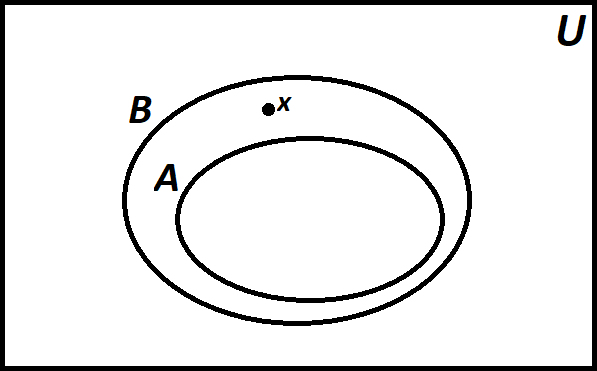
\includegraphics[width = 7 cm]{figures/sets/fig-sets-02-00.png}
      \caption{O conjunto $A$ está contido no conjunto $B$, equivalentemente, $B$ contém $A$.}
      \label{fig:sets-02-00}
  \end{figure}

  \textbf{Interseção:} Se estamos interessados em conjuntos/elementos que pertencem simultaneamente a dois conjuntos $A$ e $B$, dizemos que estamos interessados na interseção de $A$ e $B$ (denotada como $A \cap B$)$^{\ref{fig:sets-02-01}}$.
  
  \begin{figure}[hbt!]
      \centering      
      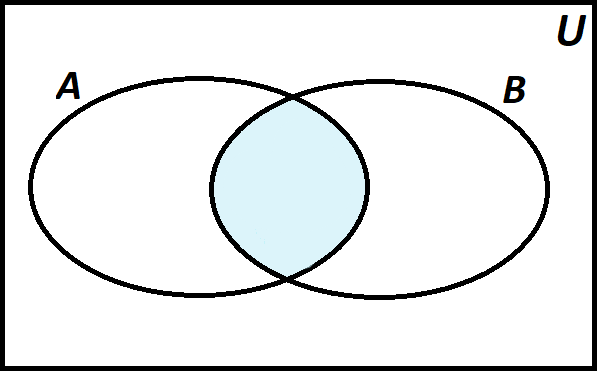
\includegraphics[width = 7 cm]{figures/sets/fig-sets-02-01.png}
      \caption{A região azul representa a visualização da interseção dos conjuntos $A$ e $B$.}
      \label{fig:sets-02-01}
  \end{figure}
  
  \textbf{União:} Já se estamos interessados nos conjuntos/elementos que fazem parte de $A$ ou de $B$ dizemos que, nosso objetivo é a união de $A$ e $B$ ($A \cup B$)$^{\ref{fig:sets-02-02}}$.
  
  \begin{figure}[hbt!]
      \centering      
      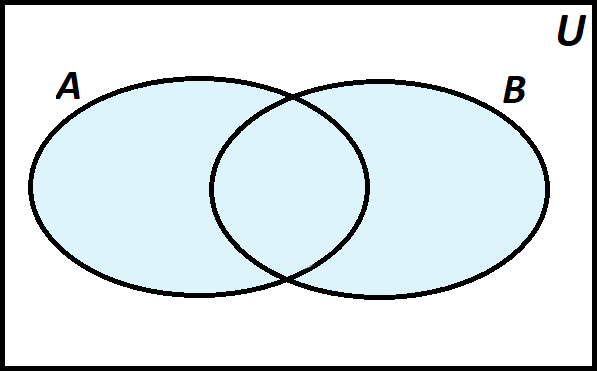
\includegraphics[width = 7 cm]{figures/sets/fig-sets-02-02.png}
      \caption{A região azul representa a visualização da união dos conjuntos $A$ e $B$.}
      \label{fig:sets-02-02}
  \end{figure}
  
  \textbf{Universo:} Quando estamos trabalhando com conjuntos é comum definirmos quem é nosso universo ($ \mathcal U $), isto é, o conjunto que conterá todos os conjuntos/elementos que estaremos trabalhando em um contexto$^{\ref{fig:sets-02-03}}$. Por exemplo, na reta real nosso universo é $\mathcal U = \mathbb{R}$.
  
  \begin{figure}[hbt!]
      \centering      
      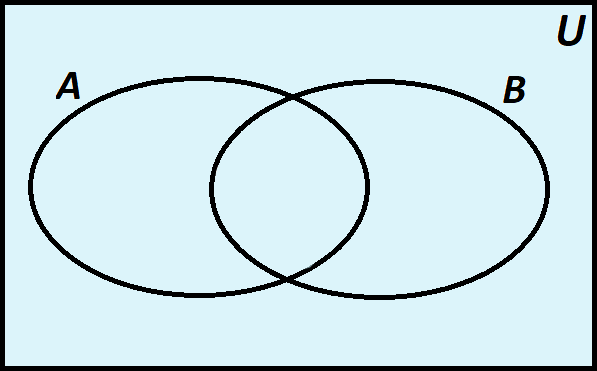
\includegraphics[width = 7 cm]{figures/sets/fig-sets-02-03.png}
      \caption{A região azul representa a visualização do nosso Universo.}
      \label{fig:sets-02-03}
  \end{figure}
  
  \textbf{Conjunto Complementar:} Sendo $A$ um conjunto, dizemos que o conjunto $A$ complementar ou complemento de $A$ (denotado como $\overline A$ ou $A^C$)contém todos os conjuntos/elementos que não estão contidos/pertencem a $A$, mas fazem parte de nosso universo ($\mathcal U$)$^{\ref{fig:sets-02-04}}$.
  
  \begin{figure}[hbt!]
      \centering      
      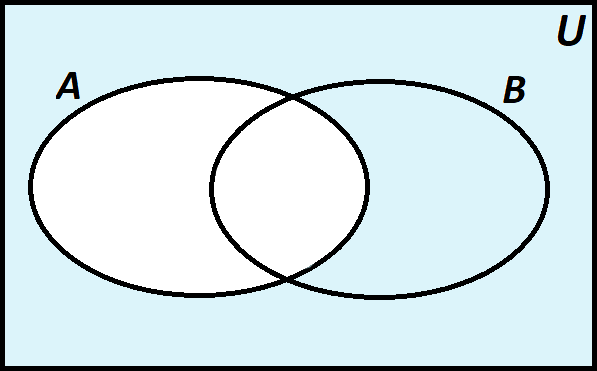
\includegraphics[width = 7 cm]{figures/sets/fig-sets-02-04.png}
      \caption{A região azul representa a visualização do complemento de $A$.}
      \label{fig:sets-02-04}
  \end{figure}
  
  \textbf{Diferença de Conjuntos :} Quando temos dois conjuntos e nosso objetivo são os conjuntos/elementos que pertencem a um destes conjuntos, mas não do outro dizemos que estamos interessados na diferença destes conjuntos. No caso, se quero os conjuntos/elementos de $B$, mas não queremos pegar os que também pertencem a $A$, queremos os elementos/conjuntos que pertencem a diferença de $B$ com $A$ (denotamos como $B-A$ ou $B \backslash A$)$^{\ref{fig:sets-02-05}}$.
  
  \begin{figure}[hbt!]
      \centering      
      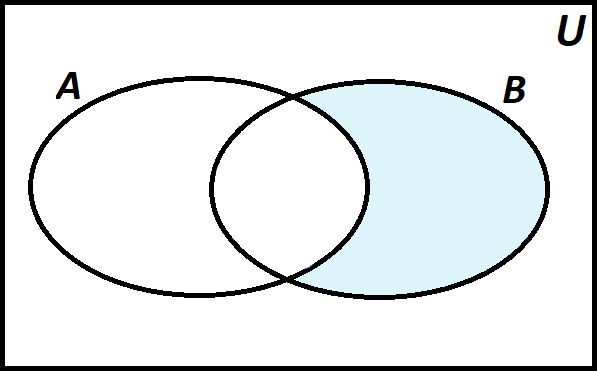
\includegraphics[width = 7 cm]{figures/sets/fig-sets-02-05.png}
      \caption{A região azul representa a visualização da diferença entre os conjuntos $B$ e $A$, isto é, a área onde estão os elementos que pertencem a $B$, mas não pertencem a $A$.}
      \label{fig:sets-02-05}
  \end{figure}
  
  Lembre-se: os diagramas apresentados servem como ferramenta auxiliar para ajudar a entender os conceitos, mas não devem ser vistos como a única ferramenta para compreender as definições e  a teoria exposta.
    
  \subsection{Definições}
  Seja $A$ e $B$ conjuntos ($\mathcal{U}$ nosso universo e $\emptyset$ o conjunto vazio, como definidos anteriormente). Assim temos, formalmente:

  \begin{itemize}
    \item \textbf{Diferença}: $A \backslash B = \{x | x \in A \land x \notin B\}$
  
    \item \textbf{Complementar}: $\overline A = \mathcal{U} \backslash A = \{x | x \in \mathcal{U} \land x \notin A\}$
  \end{itemize} 

  \subsection{Axiomas}
  Agora iremos apresentar alguns axiomas que servirão como base para todo o desenvolvimento dos conteúdos aqui propostos. Quando utilizarmos a palavra elemento, estaremos utilizando-a com a ideia de que um conjunto que pertença a outro é um elemento do segundo, para evitar repetir o uso excessivo da palavra conjunto.
  
  \textbf{Axioma da Completude:} Dois conjuntos são iguais, se e somente se, todo elemento que pertence ao primeiro conjunto pertence ao segundo e, todo elemento que pertence ao segundo também pertence ao primeiro, ou seja:
  
  \[\forall A \hspace{1.5mm} \forall B \hspace{1.5mm} (A = B) \iff (\forall x \hspace{1.5mm} (x \in A \iff x \in B))\] 
  
  Através desse axioma fica mais claro de entender duas propriedades dos conjuntos. 
  
  Deste axioma, vem a explicação do motivo de que a ordem dos elementos de um conjunto não importa. Pois dado dois conjuntos com os mesmos elementos, mas em ordem diferente (por exemplo, $X=\{a,b,c,d,e,f\}$ e o conjunto $Y=\{e,c,f,b,a,d\}$) eles ainda satisfazem a propriedade de que se $t$ pertence a um deles implica $t$ pertencer ao outro. Outro ponto interessante é que não importa se um conjunto possui elementos repetidos ele continuará igual ao que possui apenas um elemento, isto é, $X=\{a,b,d,e\}$ é igual ao $Y=\{b,a,d,a,e,b,b\}$. Ou seja, em um conjunto não importa a ordem e nem as repetições de elementos.
  
  \textbf{Axioma da Existencia do Conjunto Vazio: } Diremos que no nosso universo ($\mathbb{U}$), existe um conjunto tal que ele não contém ninguém, ou seja, ele é vazio, daí seu nome, Conjunto Vazio (denotado por $\emptyset$). O axioma é:
      
    \[\exists A \hspace{1.5mm} \forall x \hspace{1.5mm} \neg\hspace{0.5mm} (x \in A)\]
  
  \textbf{Unicidade do Conjunto Vazio}
  
  Podemos provar a unicidade do conjunto vazio a partir dos dois axiomas acimas, suponhamos que existam dois conjuntos ($A$ e $B$) com a propriedade do conjunto vazio, assim utilizando o axioma da Extensão concluíremos que eles são iguais, suponhamos $t$ arbitrário:
  
  \begin{center}
      \begin{landscape}
      \AxiomC{$\forall a  \forall b  (a = b) \iff (\forall x  (x \in a \iff x \in b))$}
      \UnaryInfC{$(A = B) \iff (\forall x  (x \in A \iff x \in B))$}
      \AxiomC{$t \in A $}
      \AxiomC{}
      \RightLabel{\scriptsize $1$}
      \UnaryInfC{$\forall x \neg (x \in A)$}
      \UnaryInfC{$\neg (t \in A)$}
      \BinaryInfC{$\perp$}
      \UnaryInfC{$t \in B$}
      \AxiomC{$t \in B$}
      \AxiomC{}
      \RightLabel{\scriptsize $1$}
      \UnaryInfC{$\forall x \neg (x \in B)$}
      \UnaryInfC{$\neg (t \in B)$}
      \BinaryInfC{$\perp$}
      \UnaryInfC{$t \in A$}
      \RightLabel{\scriptsize $\iff I_1$}
      \BinaryInfC{$t \in A \iff t \in B$}
      \UnaryInfC{$\forall x  (x \in A \iff x \in B)$}
      %\RightLabel{\scriptsize $\to E_4$}
      \BinaryInfC{A=B}
      \DisplayProof
      \end{landscape}
  \end{center}

  \textbf{Axioma do Par: } Este axioma nos diz que para todos os conjuntos $A$ e $B$, existe um conjunto conjunto que é $\{A,B\}$. Ou seja,
  
    \[\forall A \hspace{1.5mm} \forall B \hspace{1.5mm} \exists C \hspace{1.5mm} \forall x \hspace{1.5mm} (x \in C \leftrightarrow x = A \vee x = B)\]
      
  Vale ressaltar que se $A=B$, teremos $\{A,B\}=\{A,A\}=\{A\}$. A aplicação sucessiva deste axioma nos permite criar uma infinidade de conjuntos finitos. Por exemplo, $A=\emptyset$ e seja $B=\emptyset$, assim teremos $\{\emptyset\}$, sendo $B=\{\emptyset\}$, teremos agora $\{\emptyset,\{\emptyset\}\}$, agora fazendo $A=\{\emptyset\}$, teremos $\{\{\emptyset\}\}$.
  
  Não pretendemos nos aprofundar mais nos axiomas de conjuntos, dado que eles utilizarão conceitos abordados futuramente, nos capítulos de Relações, Funções e Axiomas.
  
  Mas como se pode ver em ..., podemos reduzir uma grande gama de coisas a conjuntas, assim podemos tratá-las na Teoria dos Conjuntos. Para saber mais sobre Teoria dos Conjuntos dê uma olhada em ... .

\section{Diagrama de Venn}
A maneira mais simples de entender a Teoria de Conjuntos, talvez seja o Diagrama de Venn. Criado por John Venn em 1880, esse sistema de representar graficamente conjuntos auxilia imensamente quem está começando a aprender esse assunto, principalmente para entender sobre a parte inicial de notações. Basicamente, consiste em representar num plano, o universo $\mathcal U$ como sendo um retângulo e cada conjunto $A,B,...$ como uma curva fechada simples (geralmente, círculo).
    
  \subsection{Para 1 ou 2 conjuntos}
  Começando com a ideia mais simples, a imagem abaixo representa em vermelho o conjunto $A$ dentro do universo $\mathcal U$:
  
  %\begin{figure}[h!]
  %    \centering
  %    \includegraphics{fig_set_01_01.png}
  %    \caption{Conjunto $A$ dentro de $\mathcal U$}
  %    \label{fig:fig_set_01_01}
  %\end{figure}
  
  Já sobre o conjunto complementar $A^c$, ele simplesmente é a parte que está no retângulo, mas não está no círculo, justamente o que não estava de vermelho na figura anterior.
  
  %\begin{figure}[h!]
  %    \centering
  %    \includegraphics{fig_set_01_02.png}
  %    \caption{Conjunto complementar $A^c$}
  %    \label{fig:fig_set_01_02}
  %\end{figure}
  
  Para representar que um elemento pertence ao conjunto $A$, simplesmente colocamos ele dentro do espaço delimitado pelo círculo que representa o conjunto, e para representar que um elemento nāo pertence ao conjunto $A$, fazemos o inverso.
  
  
  %\begin{figure}[h!]
  %    \centering
  %    \includegraphics{figure_set_01_03.png}
  %    \caption{$a \in A$ e $b \notin A$}
  %    \label{fig:figure_set_01_03}
  %\end{figure}
  
  Quando vamos representar mais de um conjunto em um diagrama de Venn, devemos necessariamente ter todas as possíveis relações, mas o que isso significa? Por exemplo, quando temos $2$ conjuntos $A$ e $B$, significa que devemos ter $4$ regiões representando respectivamente: elementos que pertencem somente à $A$, elementos que pertencem somente à $B$, elementos que pertencem à $A$ e à $B$ simultaneamente e elementos que não pertencem a nenhum dos conjuntos. Precisamos disso, para que tudo que provarmos para dois conjuntos $A$ e $B$, possa ser generalizado para dois conjuntos quaisquer, isso será explicado melhor num exemplo posterior.
  
  Utilizando esse artífiico, podemos representar todas as definições de intersecçāo, uniāo e diferença de $2$ conjuntos, introduzidas na seçāo anterior. Veja nas figuras abaixo:
  
  %\begin{figure}[h!]
  %    \centering
  %    \includegraphics{figure_set_01_04.png}
  %    \caption{Intersecção $A \cap B$}
  %    \label{fig:figure_set_01_04}
  %\end{figure}
  
  %\begin{figure}[h!]
  %    \centering
  %    \includegraphics{figure_set_01_05.png}
  %    \caption{União $A \cup B$}
  %    \label{fig:figure_set_01_05}
  %\end{figure}
  
  %\begin{figure}[h!]
  %    \centering
  %    \includegraphics{figure_set_01_06.png}
  %    \caption{Diferença $A \setminus B$}
  %    \label{fig:figure_set_01_06}
  %\end{figure}
  
  Todavia, isso ainda não permite fazer tudo que desejamos. Se quisermos representar que $A \subseteq B$, a ideia inicial seria colocar o círculo $A$ dentro do círculo $B$, quebrando o rigor de manter todas as possíveis relações, pois não teremos uma região para representar os elementos que pertecem somente a $A$. Então, como resolver esse problema? Representamos os conjuntos $A$ e $B$ da mesma forma que anteriormente e também escrevemos o símbolo do conjunto vazio $\emptyset$ na região dos elementos que pertencem somente a $A$. Assim, só existem elementos no conjunto $A$ que estão na região $A\cap B$, ou seja, se um elemento está em $A$, como consequência ele está em $B$, exatamente a definição de $A \subseteq B$.
  
  %\begin{figure}[h!]
  %    \centering
  %    \includegraphics{figure_set_01_07.png}
  %    \caption{Subconjunto $A \subseteq B$}
  %    \label{fig:figure_set_01_07}
  %\end{figure}
  
  É inegável que para muitos exemplos isso se torna inviável, principalmente quando o único objetivo é fazer uma ilustração matemática do problema, como por exemplo: tomamos o universo $\mathcal U$ como a fauna do nosso planeta, nele temos dois conjuntos $A$ de humanos e $B$ de mamíferos. É previamente conhecido que todos os humanos são mamíferos, falando de outra forma, que $A \subseteq B$. Logo, pra representar um problema que envolva esses elementos, podemos utilizar o \textbf{Diagrama de Euler}, similar ao Diagrama de Venn, com a diferença de que não é necessário mostrar todas as possíveis relações, mas apenas as relações específicas do problema retratado. E assim, fazer exatamente o que tinha sido proposto no parágrafo anterior e, colocar o círculo $A$ dentro do círculo $B$.

  %\begin{figure}[h!]
  %    \centering
  %    \includegraphics{figure_set_01_08.png}
  %    \caption{Diagrama de Euler $A \subseteq B$}
  %    \label{fig:figure_set_01_08}
  %\end{figure}

  \subsection{Para 3 conjuntos ou mais}    
  Já foi bastante falado sobre Diagrama de Venn, mas nem chegamos a trabalhar com mais de $2$ conjuntos, o que é importante, dado que a Teoria de Conjuntos não se resume a $A$ e $B$. Mas antes de partirmos para mais conjuntos, vamos pensar numa generalização de quantas regiões diferentes devemos ter para que o diagrama seja um Diagrama de Venn. Dado $n$ conjuntos diferentes, tomamos um elemento qualquer $x$, e para cada um dos $n$ conjuntos existem duas possibilidades: $x \in $ conjunto e $x \notin $ conjunto. Logo, concluímos que existem $\underbrace{\begin{matrix} 2\cdot2\cdots2\cdot2\end{matrix}}_{n} = 2^n$ possibilidades de pertencimento de $x$ nos conjuntos, equivalente à dizer que existem $2^n$ regiões diferentes. Isso bate perfeitamente com o caso anterior pra $2$ conjuntos, pois vimos que era necessário ter $4=2^2$ regiões diferentes.

  Agora, com $3$ conjuntos $A$, $B$ e $C$, o número de regiões diferentes é $2^3=8$, mas como iremos representá-las? A primeira ideia que vem a cabeça é adicionar um círculo representando o conjunto $C$ no diagrama da figura $\ref{fig:sets-02-00}$, intersectando as regiões já existentes, resultando na figura abaixo:

  Fazendo uma rápida contagem, obtemos $8$ regiões diferentes, exatamente como deve ser (lembrete: A região fora dos conjuntos mas dentro do universo $\mathcal U$, também é considerada na contagem). E da mesma forma que representamos bla bla bla

  \subsection{Aplicações}
  Ainda vai ter algo escrito

\section{Prova de Teoremas}
Nesta seção iremos tratar de formalizar definições e Teoremas. Ao contrário da seção $5.2$, onde o foco era transmitir a notação e uma ideia geral dos conceitos.

Aqui serão apresentadas algumas provas em Lean para o conteúdo apresentado. Não se preocupe, caso não entenda sobre o que o código quer dizer ignore ele por enquanto e após ler as próximas duas seções (que falam de conjuntos em Lean), volte e tente compreender o que foi feito. Já que o foco principal nesta parte são as provas matemáticas tradicionais e as definições mais precisas.

  \subsection{Prova Matemática Formal}
  Ainda vai ter algo escrito aqui

  \subsection{Dedução Natural}
  Ainda vai ter algo escrito aqui

\section{Conjuntos em Lean}
Embora na teoria axiomática dos conjuntos se considere conjuntos de objetos distintos, em matemática é mais comum considerar subconjuntos de algum dominio fixo ($\mathcal U $). É assim que os conjuntos são tratados em Lean. Para qualquer dado do tipo $U$, Lean nos retorna um novo dado tipo $conjunto$ $U$, que consiste no conjunto dos elementos de $U$. Assim, por exemplo, podemos raciocinar sobre conjuntos de números naturais, conjuntos de números inteiro ou conjuntos de pares de números naturais.

  \subsection{Notações}
  O lean possui uma biblioteca padrão para lidar com conjuntos chamada set e, sempre que formos utilizar um comando que pertence à ela, é necessário escrever {\fontencoding{U}\fontfamily{cmtt}\selectfont set.comando}. Entretanto, pra facilitar nossa vida, podemos escrever {\fontencoding{U}\fontfamily{cmtt}\selectfont open set} no início do código, o que permite escrevermos somente {\fontencoding{U}\fontfamily{cmtt}\selectfont comando}, e o lean já entende que ele pertence a biblioteca set.
  
  Além disso, para trabalharmos com conjuntos, também é essencial definirmos um tipo {\fontencoding{U}\fontfamily{cmtt}\selectfont U} e sabermos utilizar conjuntos e elementos desse tipo. Para isso, utilizamos o código abaixo:

  \begin{lstlisting}
  open set

  variable {U : Type}
  variables A B C : set U
  variable x : U \end{lstlisting}

  Temos aqui uma pequena lista de como se representa os principais caractéres da parte de conjuntos em Lean: 

  \begin{itemize}
      \item $\in$ $\rightarrow$ $\backslash$in
    
      \item $\notin$ $\rightarrow$ $\backslash$notin
    
      \item $\subset$ $\rightarrow$ $\backslash$subset
    
      \item $\subseteq$ $\rightarrow$ $\backslash$sub
    
      \item $\emptyset$ $\rightarrow$ $\backslash$empty
    
      \item $\cup$ $\rightarrow$ $\backslash$un \ ou \ $\backslash$cup \ ou \ $\backslash$union
    
      \item $\cap$ $\rightarrow$ $\backslash$i \ ou \ $\backslash$cap \ ou \ $\backslash$intersection
  \end{itemize}

  Obs$^{1}$.: O conjunto universal é denotado {\fontencoding{U}\fontfamily{cmtt} \selectfont univ}.

  Obs$^{2}$.: O complementar de um conjunto é denotado com um símbolo de negação antes de seu símbolo, assim: $-A$

  Podemos ver alguns exemplos abaixo:
  \begin{lstlisting}
    open set
    variable {U : Type}
    variables A B C : set U
    variable x : U

    #check x ∈ A
    #check A ∪ B
    #check B \ C
    #check C ∩ A
    #check -C
    #check ∅ ⊆ A
    #check B ⊆ univ \end{lstlisting}

  Noções básicas da teoria dos conjuntos são definidas na biblioteca principal do Lean, mas teoremas e notações adicionais que iremos utilizar nesse capítulo, estão disponíveis em uma biblioteca auxiliar que é carregada com o comando 
  {\fontencoding{U}\fontfamily{cmtt} \selectfont import data.set}, o qual deve aparecer no início do arquivo.

  \begin{lstlisting}
    import data.set
    open set
    variable {U : Type}
    variables A B C : set U
    variable x : U \end{lstlisting}

  A partir desse momento, para evitar repetição, iremos omitir as $4$ primeiras linhas do código, no entanto \textbf{você deve lembrar que elas existem para seu código funcionar.} Já sobre a linha $5$, não é necessário escrever nos próximos exemplos, pois sempre iremos se referenciar a um elemento do tipo{\fontencoding{U}\fontfamily{cmtt} \selectfont U}, dentro de {\fontencoding{U}\fontfamily{cmtt}\selectfont example, lemma} ou {\fontencoding{U}\fontfamily{cmtt}\selectfont theorem}.

  \subsection{Primeiros Passos}

  Relembrando a definição de subconjunto, podemos utilizar o template abaixo para mostrar que o conjunto $A$ é um subconjunto de $B$:

  \begin{lstlisting}
  example : A ⊆ B :=
  assume x : U,
  assume h : x ∈ A,
  show x ∈ B, from sorry \end{lstlisting}

  Obs: Na linha $2$ poderíamos ter escrito somente {\fontencoding{U}\fontfamily{cmtt}\selectfont assume x}, pois já inferiria que {\fontencoding{U}\fontfamily{cmtt}\selectfont x} é do tipo {\fontencoding{U}\fontfamily{cmtt}\selectfont U}.

  Já para mostrar que $A$ e $B$ são iguais, temos dois comandos diferentes: {\fontencoding{U}\fontfamily{cmtt}\selectfont eq\_of\_subset\_of\_subset} e {\fontencoding{U}\fontfamily{cmtt}\selectfont ext}.

  \textbf{eq\_of\_subset\_of\_subset:} Ele funciona interpretando a seguinte expressão $(A \subseteq B \wedge B \subseteq A) \Rightarrow A=B$, ou seja, obtém a equivalência dos conjuntos a partir do fato de que o primeiro é subconjunto do segundo, e vice-vera. Veja o código:

  \begin{lstlisting}
  example : A = B :=
  eq_of_subset_of_subset
    (assume x,
      assume h : x ∈ A,
      show x ∈ B, from sorry)
    (assume x,
      assume h : x ∈ B,
      show x ∈ A, from sorry) \end{lstlisting}

  \textbf{ext:} É uma sigla para ``extensionality", ou seja, extensionalidade. Matemáticamente, isso representa a expressão $\forall x \ (x \in A \leftrightarrow x \in B) \Rightarrow A=B$. Veja o código:

  \begin{lstlisting}
  example : A = B :=
  ext (assume x, iff.intro
    (assume h : x ∈ A,
      show x ∈ B, from sorry)
    (assume h : x ∈ B,
      show x ∈ A, from sorry)) \end{lstlisting}

  Além disso, o Lean possui interpretação ambígua para regras de união, interseção e outras operações em conjuntos que são consideradas “definições”. Isso significa que as expressões $x$ $\in$ $A$ $\cap$ $B$ e $x$ $\in$ $A$ $\wedge$ $x$ $\in$ $B$ possuem a mesma interpretação no Lean. Isso também é válido para outras construções em conjuntos, como: $x$ $\in$ $A$ $\backslash $ $B$ e $x$ $\in$ $A$ $\wedge$ $\neg$ $(x$ $\in$ $B)$. O termo $\neg$ $(x$ $\in$ $B)$ é somente outra forma de escrever $x$ $\notin$ $B$. Abaixo são apresentadas algumas aplicações dessa interpretação:

  \begin{lstlisting}
  example : ∀ x, x ∈ A → x ∈ B → x ∈ A ∩ B :=
  assume x,
  assume h₁ : x ∈ A,
  assume h₂ : x ∈ B,
  show x ∈ A ∩ B, from and.intro h₁ h₂

  example : A ⊆ A ∪ B :=
  assume x,
  assume h : x ∈ A,
  show x ∈ A ∪ B, from or.inl h

  example : ∅ ⊆ A  :=
  assume x,
  assume h : x ∈ (∅ : set U),
  show x ∈ A, from false.elim h \end{lstlisting}

  Observe no último exemplo a necessidade de usar a notação {\fontencoding{U}\fontfamily{cmtt} \selectfont ($\emptyset$ : set U)}, dizendo ao nosso provador que o $\emptyset$ é um conjunto de {\fontencoding{U}\fontfamily{cmtt}
  \selectfont U}. Isso acontece pois ele não consegue inferir que tipo é o conjunto vazio, dado que por definição, esse conjunto existe em qualquer universo, ou seja, pode ser de qualquer tipo.

  Opcionalmente, podemos usar alguns teoremas da biblioteca {\fontencoding{U}\fontfamily{cmtt}
  \selectfont data.set}, projetados especificamente para uso em conjuntos:

  \begin{lstlisting}
  example : ∀ x, x ∈ A → x ∈ B → x ∈ A ∩ B :=
  assume x,
  assume : x ∈ A,
  assume : x ∈ B,
  show x ∈ A ∩ B, from mem_inter ‹x ∈ A› ‹x ∈ B›

  example : A ⊆ A ∪ B :=
  assume x,
  assume h : x ∈ A,
  show x ∈ A ∪ B, from mem_union_left B h

  example : ∅ ⊆ A  :=
  assume x,
  assume : x ∈ ∅,
  show x ∈ A, from absurd this (not_mem_empty x) \end{lstlisting}

  Lembre-se que o comando{\fontencoding{U}\fontfamily{cmtt}
  \selectfont absurd} pode ser usado para provar qualquer fato a partir de duas hipóteses contrárias: $h_1$ : $P$ e $h_2$ : $\neg$ $P$. 

  Aqui, o teorema {\fontencoding{U}\fontfamily{cmtt}
  \selectfont not\_mem\_empty x} significa $x$ $\notin$ $\emptyset$. Para ver a declaração de teoremas disponíveis, utilize o comando{\fontencoding{U}\fontfamily{cmtt}
  \selectfont \#check}:

  \begin{lstlisting}
  #check @mem_inter
  #check @mem_of_mem_inter_left
  #check @mem_of_mem_inter_right
  #check @mem_union_left
  #check @mem_union_right
  #check @mem_or_mem_of_mem_union
  #check @not_mem_empty \end{lstlisting}

  Neste caso, o símbolo{\fontencoding{U}\fontfamily{cmtt}
  \selectfont @} impede que ele tente preencher argumentos implícitos automaticamente, forçando-o a exibir a declaração completa do teorema.

  Já que podemos relacionar conjuntos com suas definições lógica, isso auxilia a comprovação de inclusões entre conjuntos:

  \begin{lstlisting}
  example : A \ B ⊆ A :=
  assume x,
  assume : x ∈ A \ B,
  show x ∈ A, from and.left this

  example : A \ B ⊆ -B :=
  assume x,
  assume : x ∈ A \ B,
  have x ∉ B, from and.right this,
  show x ∈ -B, from this \end{lstlisting}

  Novamente, é possível usar versões dos teoremas projetados especificamente para conjuntos:

  \begin{lstlisting}
  example : A \ B ⊆ A :=
  assume x,
  assume : x ∈ A \ B,
  show x ∈ A, from mem_of_mem_diff this

  example : A \ B ⊆ -B :=
  assume x,
  assume : x ∈ A \ B,
  have x ∉ B, from not_mem_of_mem_diff this,
  show x ∈ -B, from this \end{lstlisting}

  %Acho que a partir desse ponto, não é necessário ter nesse capítulo. Talvez seja melhor deixar só pro capítulo de propriedades. Por isso, já copiei e colei no outro capítulo. Se ainda sim quiser falar sobre como lidar com sorry, pegue algum dos exemplos já citados acima. E se quiser colocar mais coisas teóricas ou explicativas, está totalmente livre. Mas deixe as propriedades/identidades pro capítulo delas.

\section{Cálculo em Conjuntos}
Ainda vai ter algo escrito aqui

  \subsection{Cálculo Matemático}
  Ainda vai ter algo escrito aqui

  \subsection{Calc em Lean}
  Ainda vai ter algo escrito aqui

\section{Propriedades}
A seguir teremos algumas propriedades e a prova do porque estão corretas.
    
\begin{itemize}  
    \item $A \cup \overline A = \mathbb{U}$
\end{itemize} 

\textbf{Prova:} Seja $x$ um elemento de $A \cup \overline A$, assim temos que 
\[x \in (A \cup \overline A)\]
\[ \iff x \in A \vee x \in \overline A\]
    
\begin{itemize}
    \item $A \cap \overline A = \empty{U}$
\end{itemize} 

\textbf{Prova:} Seja $x$ um elemento de $A \cap \overline A$, assim:

$(i)$ Provaremos que $ \forall x (x \in A \cap \overline A) \rightarrow \forall x  (x \in \emptyset) $ :

\begin{center}
    \AxiomC{}
    \RightLabel{\scriptsize $1$}
    \UnaryInfC{$ \forall x (x \in A \cap \overline A)$}
    \UnaryInfC{$t \in A \cap \overline A$}
    \UnaryInfC{$t \in A \land t \in \overline A $}
    \UnaryInfC{$t \in A $}
    \AxiomC{}
    \RightLabel{\scriptsize $1$}
    \UnaryInfC{$ \forall x (x \in A \cap \overline A)$}
    \UnaryInfC{$t \in A \cap \overline A$}
    \UnaryInfC{$t \in A \land t \in \overline A $}
    \UnaryInfC{$t \in \overline A $}
    \UnaryInfC{$t \in \mathbb{U} \land t \notin A $}
    \UnaryInfC{$t \notin A $}
    \BinaryInfC{$\perp$}
    \UnaryInfC{$t \in \emptyset$}
    \UnaryInfC{$\forall x  (x \in \emptyset)$}
    \RightLabel{\scriptsize $1$}
    \UnaryInfC{$ \forall x (x \in A \cap \overline A) \rightarrow \forall x  (x \in \emptyset) $}
    \DisplayProof
\end{center}
    
$(ii)$ Provaremos que $ \forall x  (x \in \emptyset) \rightarrow \forall x (x \in A \cap \overline A)$ :
\begin{center}
    \AxiomC{}
    \RightLabel{\scriptsize $1$}
    \UnaryInfC{$\forall x  (x \in \emptyset)$}
    \UnaryInfC{$\perp$}
    \UnaryInfC{$t \in A \cap \overline A$}
    \UnaryInfC{$ \forall x (x \in A \cap \overline A)$}
    \RightLabel{\scriptsize $1$}
    \UnaryInfC{$\forall x  (x \in \emptyset) \rightarrow \forall x (x \in A \cap \overline A)$}
    \DisplayProof
\end{center}

Portanto, de $(i)$ e $(ii)$, concluímos que $ \forall x (x \in A \cap \overline A) \iff \forall x  (x \in \emptyset) $, ou seja, $A \cap \overline A$.

%Renan
Como o Lean tem que desenvolver definições, ele pode acabar se confundindo às vezes. Por exemplo, na prova a seguir, se você subtituir a última linha por{\fontencoding{U}\fontfamily{cmtt}
\selectfont sorry}, o Lean terá problemas tentando entender que você quer que ele desenvolva o símbolo de subconjunto:

\begin{lstlisting}
example : A ∩ B ⊆ B ∩ A :=
assume x,
assume h : x ∈ A ∩ B,
have h₁ : x ∈ A, from and.left h,
have h₂ : x ∈ B, from and.right h,
and.intro h₂ h₁ \end{lstlisting}

Uma solução alternativa é usar o comando{\fontencoding{U}\fontfamily{cmtt}
\selectfont show}. Na maioria das vezes, fornecer informações adicionais para o Lean pode ser útil. Outra solução é nomear um teorema, o que leva o Lean a usar um método um pouco diferente de processar a prova, corrigindo o problema como um efeito colateral de sorte.

\begin{lstlisting}
example : A ∩ B ⊆ B ∩ A :=
assume x,
assume h : x ∈ A ∩ B,
have h₁ : x ∈ A, from and.left h,
have h₂ : x ∈ B, from and.right h,
show x ∈ B ∩ A, from sorry

theorem my_example : A ∩ B ⊆ B ∩ A :=
assume x,
assume h : x ∈ A ∩ B,
have h₁ : x ∈ A, from and.left h,
have h₂ : x ∈ B, from and.right h,
sorry \end{lstlisting}

Parte de Identidade de Conjuntos: Nessa seção, falaremos brevemente sobre Identidades de conjuntos.

Iniciaremos com um exemplo simples: a regra da distributividade para conjuntos: $A \cup (B \cap C)$ = $(A \cup B) \cap (A \cup C)$. Uma maneira de prova-la é:


\begin{lstlisting}
import data.set
open set

variable {U : Type}
variables A B C : set U

example : A ∪ (B ∩ C) = (A ∪ B) ∩ (A ∪ C) :=
eq_of_subset_of_subset
  (assume x,
    assume h : x ∈ A ∪ (B ∩ C),
    or.elim h
      (assume h₁ : x ∈ A,
        have h₂ : x ∈ A ∪ B, from or.inl h₁,
        have h₃ : x ∈ A ∪ C, from or.inl h₁,
        show x ∈ (A ∪ B) ∩ (A ∪ C), from and.intro h₂ h₃)
      (assume h₁ : x ∈ B ∩ C,
        have h₂ : x ∈ B, from and.left h₁,
        have h₃ : x ∈ C, from and.right h₁,
        have h₄ : x ∈ A ∪ B, from or.inr h₂,
        have h₅ : x ∈ A ∪ C, from or.inr h₃,
        show x ∈ (A ∪ B) ∩ (A ∪ C), from and.intro h₄ h₅))
  (assume x,
    assume h : x ∈ (A ∪ B) ∩ (A ∪ C),
    have h₁ : x ∈ A ∪ B, from and.left h,
    have h₂ : x ∈ A ∪ C, from and.right h,
    or.elim h₁
      (assume h₃ : x ∈ A,
        show x ∈ A ∪ (B ∩ C), from or.inl h₃)
      (assume h₃ : x ∈ B,
      or.elim h₂
        (assume h₄ : x ∈ A,
        show x ∈ A ∪ (B ∩ C), from or.inl h₄)
        (assume h₄ : x ∈ C,
        have h₅ : x ∈ B ∩ C, from and.intro h₃ h₄, 
        show x ∈ A ∪ (B ∩ C), from or.inr h₅)))
\end{lstlisting}

Outra identidade que usaremos como exemplo aqui é a Lei de Absorção:  

\begin{center}
    $A \cup (A \cap B) = A$
\end{center}

Nos templates abaixo temos duas formas de escrever a prova: a que estamos utilizando ao longo deste capítulo; e em forma de lógica booleana, trocando o sinal de igual pelo de equivalência, ou ``se e somente se", ($\leftrightarrow$). (Você consegue reprentá-lo no Lean escrevendo: $\backslash$iff ou $\backslash$lr)

\begin{lstlisting}
import data.set
open set

theorem inter_subseq (H : Type)(P Q : set H) : P ∩ (P ∪ Q) = P :=
eq_of_subset_of_subset
  (assume x,
    assume h : x ∈ P ∩ (P ∪ Q),
    show x ∈ P, from h.left)
  (assume x,
    assume h : x ∈ P,
    have h₁ : x ∈ P ∪ Q, from or.inl h,
    show x ∈ P ∩ (P ∪ Q), from and.intro h h₁)

variable  U : Type
variables A B : set U

example : A ∪ (A ∩ B) = A :=
calc
  A ∪ (A ∩ B) = (A ∪ A) ∩ (A ∪ B) : by rw union_distrib_left
          ... = A ∩ (A ∪ B)       : by rw union_self
          ... = A                 : by rw inter_subseq
\end{lstlisting}

\begin{lstlisting}
import logic.basic
open classical

theorem left_of_and (P Q : Prop) : P ∧ (P ∨ Q) ↔ P :=
iff.intro
  (assume h : P ∧ (P ∨ Q),
  show P, from h.left)
  (assume h : P,
  have h₁ : P ∨ Q, from or.inl h,
  show P ∧ (P ∨ Q), from and.intro h h₁)

variables A B : Prop

example : A ∨ (A ∧ B) ↔ A :=
calc
  A ∨ (A ∧ B) ↔ (A ∨ A) ∧ (A ∨ B) : by rw or_and_distrib_left
          ... ↔ A ∧ (A ∨ B)        : by rw or_self
          ... ↔ A                  : by rw left_of_and
\end{lstlisting}

  \subsection{Básicas}
  %Pode ser separada em: Básicas, Sobre o conjunto vazio, Sobre o Universo
  Ainda vai ter algo escrito aqui

  \subsection{Comutatividade}
  Ainda vai ter algo escrito aqui

  \subsection{Associatividade}
  Ainda vai ter algo escrito aqui

  \subsection{Distributividade}
  Ainda vai ter algo escrito aqui

  \subsection{Complementar/Lei de Demorgan}
  Ainda vai ter algo escrito aqui

  \subsection{Lei da Absorção}
  Ainda vai ter algo escrito aqui

  \subsection{Extras}
  Ainda vai ter algo escrito aqui

\section{Famílias Indexadas}

  \subsection{Definição}
  Ainda vai ter algo escrito aqui

  \subsection{Em Lean}
  Ainda vai ter algo escrito aqui

\section{Power Set}

  \subsection{Definição}
  Ainda vai ter algo escrito aqui

  \subsection{Em Lean}
  Ainda vai ter algo escrito aqui

\section{Exercícios}
\begin{enumerate}
    
\item Questões de Identidades de conjuntos
    
\begin{lstlisting}
import data.set
open set

section
  variable U : Type
  variables A B C : set U

--Comutatividade em ∩ e ∪ 
  example : A ∩ B = B ∩ A := 
  eq_of_subset_of_subset
    (assume x,
        assume h : x ∈ A ∩ B,
        have h₁ : x ∈ A, from h.left,
        have h₂ : x ∈ B, from h.right,
        show x ∈ B ∩ A, from and.intro h₂ h₁)
    (assume x,
        assume h : x ∈ B ∩ A,
        have h₁ : x ∈ B, from h.left,
        have h₂ : x ∈ A, from h.right,
        show x ∈ A ∩ B, from and.intro h₂ h₁)

  example : A ∪ B = B ∪ A:=
  eq_of_subset_of_subset
    (assume x,
        assume h : x ∈ A ∪ B,
        or.elim h
        (assume h₁ : x ∈ A,
        show x ∈ B ∪ A, from or.inr h₁)
        (assume h₁ : x ∈ B,
        show x ∈ B ∪ A, from or.inl h₁))
    (assume x,
        assume h : x ∈ B ∪ A,
        or.elim h
        (assume h₁ : x ∈ B,
        show x ∈ A ∪ B, from or.inr h₁)
        (assume h₁ : x ∈ A,
        show x ∈ A ∪ B, from or.inl h₁))

--Associatividade
  example : (A ∩ B) ∩ C = A ∩ (B ∩ C) :=
  eq_of_subset_of_subset
    (assume x,
        assume h : x ∈ (A ∩ B) ∩ C,
        have h₁ : x ∈ A ∩ B, from h.left,
        have h₂ : x ∈ B ∩ C, from and.intro h₁.right h.right,
        show x ∈ A ∩ (B ∩ C), from and.intro h₁.left h₂) 
    (assume x,
        assume h : x ∈ A ∩ (B ∩ C),
        have h₁ : x ∈ B ∩ C, from h.right,
        have h₂ : x ∈ A ∩ B, from and.intro h.left h₁.left,
        show x ∈ (A ∩ B) ∩ C, from and.intro h₂ h₁.right) 

--De Morgan
  open classical 
  example : -(A ∩ B) = -A ∪ -B :=
    ext $
    assume x,
    iff.intro
        (assume h₁ : x ∈ -(A ∩ B),
            have g₁ : x ∈ (A ∪ -A), from em (x ∈ A),
            have g₂ : x ∈ (B ∪ -B), from em (x ∈ B),
            or.elim g₁
                (assume h₂ : x ∈ A, or.elim g₂
                    (assume h₃ : x ∈ B, show x ∈ -A ∪ -B,
                        from false.elim (h₁ ⟨h₂,h₃⟩))
                    (assume h₃ : x ∈ -B, show x ∈ -A ∪ -B,
                        from or.inr h₃))
                (assume h₂ : x ∈ -A, show x ∈ -A ∪ -B,
                    from or.inl h₂))

        (assume h₁ : x ∈ -A ∪ -B,
            assume h₂ : x ∈ (A ∩ B), show false,
            from or.elim h₁
                (assume h₃ : x ∈ -A, h₃ h₂.left )
                (assume h₃ : x ∈ -B, h₃ h₂.right))

  example : -(A ∪ B) = -A ∩ -B :=
    ext $
    assume x,
    iff.intro
        (assume h₁ : x ∈ -(A ∪ B),
            have g₁ : x ∈ -A, from
            assume h₂ : x ∈ A,
                have h₃ : x ∈ A ∪ B,
                from or.inl h₂, (h₁ h₃),
            have g₂ : x ∈ -B, from
            assume h₂ : x ∈ B,
                have h₃ : x ∈ A ∪ B,
                from or.inr h₂, (h₁ h₃),
            show x ∈ -A ∩ -B, from ⟨g₁, g₂⟩)

        (assume h₁ : x ∈ -A ∩ -B,
            show x ∈ -(A ∪ B), from
            assume h₂ : x ∈ A ∪ B,
            or.elim h₂
                (assume h3 : x ∈ A, h₁.left h3)
                (assume h3 : x ∈ B, h₁.right h3))
end 
\end{lstlisting}

\item Prove que $A \cup \overline A = \mathcal U$. (Fornecendo uma prova tradicional e uma em Lean.)

\textbf{Resposta} 




\item Questões com calc
    
    
\end{enumerate}

\chapter{Relações}
Em capítulos anteriores, discutimos proposições que lidavam com a relação entre objetos matemáticos. Muitas vezes na matemática, e mesmo no contexto em que estamos inseridos, estamos interessados em definir e estudar relações entre objetos distintos. Por exemplo, podemos estar interessados em certas própriedades sobre a relação \textit{é vais velho que}, entre seres vivos, e diremos que essa é uma relação \textit{irreflexiva}, \textit{transitiva}, ou ainda, uma relação de \textit{ordem estrita}.

Nesse capítulo discutimos exatamente essas noções, e definimos certos tipos de relaçõs mais comuns.

\section{Semântica das Relações}
Podemos abstrair a noção semântica de relação para um universo $R$ de tuplas de aridade definida, que contem a sequencia dos objetos relacionados. Por exemplo, considere que o elemento $a$ está relacionado a $b$ por uma relação $R$. Ppodemos denotar $aRb$, ou $R(a,b)$ significando que o par $(a,b)\in R$, está definido como existente no universo daquela relação. Como se pode esperar, a relação pode ter qualquer aridade necessária, e relacionar objetos de tipos distintos.

Considere, a partir disso, o universo de objetos $u = \{Ana, Bia, Cid\}$, e a relação \textit{conhece}, definida por $U\times U \supseteq A = \{(Ana, Bia), (Bia, Cid)\}$. Podemos dizer que \textit{Bia conhece Ana}?

%\section{Definições}
\theoremstyle{definition}
\newtheorem{definition}{Definição}[section]

%\theoremstyle{definition}
%\newtheorem{example}{Exemplo}[section]

\theoremstyle{plain}
\newtheorem{theorem}{Proposição}[section]

%\theoremstyle{plain}
%\newtheorem{corollary}{Corolário}[section]

Definimos uma série de tipos de relações importantes, frequentemente encontradas na literatura.
Note que muitas das definições se aplicam a relações conhecidas como \textit{maior que}, nos naturais, ou \textit{pertence} para conjuntos.

\section{Relações de Ordem}
Discutimos uma classe de relações binárias importantes: as chamadas relações de ordem.
Aqui, definimos relações de\textit{parciais} ou \textit{estritas}.
Usaremos os símbolos $\leq$ e $<$ para nos referir a relações quaisquer entre elementos de alguma estrutura $A$, e os usamos infixados: $x \leq y$ ou $x < y$.

\begin{definition}
    \label{partial_order}
    Seja $\leq$ uma relação. Dizemos que $\leq$ é de \textit{ordem parcial} se respeita as seguintes propriedades:

    \begin{itemize}
        \item \textbf{reflexividade:} para todo $x \in A$, $x\leq x$.
        \item \textbf{transitividade:} para todo $xy,z \in A$, se $x\leq y$, e $yleq z$, então $x\leq z$.
        \item \textbf{antissimetria:} para todo $x,y \in A$, se $x\leq y$ e $y \leq x$, então $x=y$.
    \end{itemize}
\end{definition}

\noindent Note que se entendemos $\leq$ por um predicado binário, as definições acima são facilmente expressos em lógica de primeira ordem.
Exemplos desse tipo são: $\leq$ em $\mathbb{N}$, $\mathbb{Z}$, $\mathbb{Q}$, e $\mathbb{R}$ ou a inclusão $\supseteq$ para a classe dos conjuntos.

Há ainda uma classe especial de relações de ordem vistas a seguir:

\begin{definition}
    \label{partial_order_total}
    Dizemos que a relação de \textit{ordem parcial} $\leq$ é \textit{total} se:

    \begin{itemize}
        \item para todo $x, y \in A$, $x\leq y$ ou $y\leq x$.
    \end{itemize}
\end{definition}

\noindent Vale observar que nos exemplos anteriores, apenas $\leq$ é total.
De fato, tome $A = \mathcal{P}(\mathbb{N}) $, os conjuntos $x={3}$ e $y={5}$ subconjuntos de $A$; claramente não vale a completude de $\subseteq$ em $A$. % Ainda, as relações \textit{divide}, $x|y$, nos inteiros, e outras...

O que dizer, no entanto, das relações \textit{menor} ou \textit{pertence}? De fato, essas pertencem a classe a seguir, as chamadas relações de \textit{ordem estrita}:

\begin{definition}
    \label{estrict_order}
    Considere $<$ relação em um conjunto $A$. Dizemos que a relação é de \textit{ordem estrita} $\leq$ é \textit{total} se:

    \begin{itemize}
        \item \textbf{transitividade: } para todo $x,y,z \in A$, se $x<y$ e $y<z$ então $x<z$.
        \item \textbf{irreflexividade: } para todo $x\in A$, $x\nless x$.
    \end{itemize}
    dizemos, ainda, que essa relação estrita é total em $A$ se:
    \begin{itemize}
        \item \textbf{tricotomia:} para todo $x,y \in A$, vale $x<y$, $x>y$ ou $x=y$.
    \end{itemize}
\end{definition}

\noindent Novamente, é facil ver como formalizar essas noções utilizando proposições em lógica de primiera ordem.

% uma relação estrita é assimétrica: prova.

A seguir, discutimos um resultado intuitivo que estabelece uma ligação importante entre as relações de ordem \textit{parciais} e \textit{estritas}:

\begin{theorem}
    \label{estrict_by_partial}
    Considere $\leq$ parcial em $A$. Podemos definir uma relação estrita $<$ em $A$, em que $x<y$ significa que $x\leq y$ e $x \neq y$. Ainda, se $\leq $ for total, então $<$ também será total.
\end{theorem}
\begin{theorem}
    \label{partial_by_estrict}
    Considere $<$ estrita em $A$. Podemos definir a relação de ordem parcial $\leq $ em $A$, em que $x\leq y$ significa que $x < y$ ou $x = y$. Ainda, se $<$ for total, então $\leq$ também será total.
\end{theorem}

\begin{proof}
    Exercício para o leitor!
\end{proof}

\section{Relações de Equivalência}
%Descrevemos as propriedades que definem esse tipo de relação, e damos exemplos. Mostramos as notações $a\sim b $, $a\equiv b$. Sugiro as relações de equivalencia "paralelo a", "modulo n", "mesma idade".


\subsection{Equivalencia e Igualdade}
Apenas discutimos brevemente como e porque Equivalencia e Igualdade são animais completamente diferentes. Toma os exemplos acima pra discutir.

\section{Relações em Lean}

\section{Exercícios}

\chapter{Funções}

Desde o final do século XIX, diversas áreas da matemática
estudam consistentemente \textit{\hyperlink{chapter.4}{conjuntos}},
\textit{\hyperlink{chapter.5}{relações}}, já apresentadas
nesse texto, e funções. Neste capítulo, debruçaremos nossa
atenção nas propriedades dessa terceira área.

Entende-se que uma função $f$ é um mapeamento entre um
domínio $X$ e um domínio $Y$, este que será conhecido como
contradomínio, posteriormente. Entretanto, para teóricos
de conjuntos, esses domínios são simplesmente considerados
conjuntos. Vimos que \textit{\hyperlink{chapter.2}{Lean}} é uma
linguagem baseada em Tipos. Dessa forma, estabelece-se uma
diferença clara entre o Domínio $X$, caracterizado pelos Tipos, e
o Conjunto $A$, que é do tipo (sub)conjunto de $X$. Em Lean:
\begin{lstlisting}
variable X : Type
variable A : set X
\end{lstlisting}

Entretanto a visão da função como mapeamento entre conjuntos
é comum entre os matemáticos e será considerada nesse texto,
fazendo as devidas comparações com a linguagem de referência,
o Lean.

\section{O Conceito de Função}

Considere dois conjuntos quaisquer $X$ e $Y$ e um mapeamento $f$
do conjunto $X$ para o conjunto $Y$. Se $f$ atribui um e apenas
um valor para cada elemento de $X$, dizemos que $f$ é uma função total, e
escrevemos $f: X \to Y$.  Chamamos $X$ de domínio de $f$, enquanto
$Y$ é o contradomínio de $f$ e $\forall x, (x \in X  \Rightarrow f(x) \in Y)$.
Nesse sentido, $\forall x_1 \in X, \forall x_2 \in X, x_1 = x_2 \Rightarrow f(x_1) = f(x_2)$.
Uma função também pode ser parcial quando ela não é definida para alguns valores
do domínio. Como toda função parcial é total ao restringir o domínio, trateremos
nesse texto das funções totais.

A maneira mais simples de se representar uma função é escrevê-la explicitamente
para cada elemento do domínio. Por exemplo, podemos escrever as seguintes expressões:

\begin{itemize}
    \item Seja $f: \mathbb{N} \to \mathbb{N}$ definida por
    $f(n) = 2\cdot n + 1$
    \item Seja $g : \mathbb{N} \to \mathbb{R}$ definida por
    $g(n) = \frac{n}{n+1}$
    \item Seja $h : \mathbb{R} \to \{0,1\}$ definida por
    $$\left \{ \begin{array}{c}
    h(x) = 1 ~if~x \in \mathbb{Q} \\
    h(x) = 0 ~ if ~ x \not \in \mathbb{Q} \\
    \end{array}
    \right. $$
 \end{itemize}

A questão que se levanta é: o que torna uma expressão explícita legítima?
Neste momento, deixaremos essa questão de lado e notaremos que a matemática
é confortável com diversos tipos de definições, como, por exemplo, a definição
de $h(x)$ no exemplo acima. Nesse mesmo exemplo, não fica claro em como podemos
definir algoritmicamente se um número real de entrada é um número racional ou não.
Porém, esse não é o objetivo do capítulo.

Note que a escolha das variáveis $x$ e $n$ são arbitrárias.
Isto nos leva à definição no capítulo de \textit{\hyperlink{chapter.4}{FOL}} de
variável ligada (\textit{bound}), visto que se renomearmos $x$ com $y$, os valores
continuam os mesmos.

Lógicos frequentemente utilizam a notação $\lambda x e(x)$ para denotar a função
que mapeia $x$ para $e(x)$. Essa notação chama-se \textit{notação lambda} e pode
ser usada da seguinte forma: $f = \lambda x(x + 1)$, que significa $f(x) = x + 1$.
Essa notação é mais interessante para cientistas da computação e lógicos do que
propriamente para matemáticos. Em Lean, definimos da seguinte forma:

\begin{lstlisting}
variables X Y : Type
variable f : X → Y
\end{lstlisting}

Lembre-se que diferenciamos o tipo $X$ do tipo $set~X$ em Lean.

\section{Primeiras Definições}

\theoremstyle{definition}
%\newtheorem{definition}{Definição}[section]

\theoremstyle{definition}
\newtheorem{example}{Exemplo}[section]

\theoremstyle{plain}
%\newtheorem{theorem}{Proposição}[section]

\theoremstyle{plain}
\newtheorem{corollary}{Corolário}[section]

\begin{definition}
    \label{def1}
    Seja um conjunto $X$. A função identidade de $A$ é a função
    $i_A : A \rightarrow A$ definida para todos os valores $x \in A$ tal que $i_A(x) = x$.
\end{definition}

\begin{definition}
    \label{def2}
    Sejam $f : X \rightarrow Y$ e $g : Y \rightarrow Z$ funções.
    Defina $k : X \rightarrow Z$ por $k(x) = g(f(x))$. A função $k$ é chamada de composição
    de $f$ e $g$ ou $f$ composta com $g$ e é escrita $g \circ f$. Desta forma, para cada elemento,
    primeiro  avaliamos $f(x) \in Y$ e depois avaliamos $g(f(x)) \in Z$.
\end{definition}

Podemos ver em Lean as definições de composição e de identidade. Note que estamos em um namespace
hidden para que não haja conflito de definições.

\begin{lstlisting}
namespace hidden
    variables {X Y Z : Type}

    def comp (f : Y → Z) (g : X → Y) : X → Z :=
    λx, f (g x)

    infixr  ` ∘ ` := comp

    #check @comp

    def id (x : X) : X := x

    #check @id

end hidden
\end{lstlisting}

\begin{definition}
    \label{def3}
    Considere $f,g : X \to Y$. Dizemos que essas funções são iguais,
    quando para todos os valores do domínio $X$, a correspondência no contradomínio $Y$ é a
    mesma. Em lógica simbólica, $\forall x (x \in X \to (f(x) = g(x)) \iff f = g $.
\end{definition}

Obseve que em termos de lógica formal de tipos, poderíamos reescrever como
$\forall x : X (f(x) = g(x)) \iff f = g$. Escrevemos essa equivalência entre lógica e funções
utilizando a extensionalidade das funções, muito semelhante à descrita no capítulo de
\textit{\hyperlink{chapter.5}{conjuntos}}. Por exemplo, se $f, g : \mathbb{R} \to \mathbb{R}$
definidas por $f(x) = x + 1$ e $g(x) = 1 + x$, então $f = g$, pois para cada valor de $x$, vale
a comutativade da soma.

Em lean, o comando \lstinline{funext} (de "function extensionality") prova a igualdade de funções.

\begin{lstlisting}
variables {X Y : Type}

example (f g : X → Y) (h : ∀ x, f x = g x) : f = g :=
    funext h
\end{lstlisting}

\begin{theorem}
    \label{prop1}
    Para todo $f: X \to Y$, $f \circ i_X = f$ e $i_Y \circ f = f$
\end{theorem}
\begin{proof}
    Seja $x$ um elemento qualquer de $X$. Então $(f \circ i_X)(x) = f(i_X(x)) = f(x)$
     e $(i_Y \circ f)(x) = i_Y(f(x)) = f(x)$, o que mostra a igualdade.
\end{proof}

No Lean, podemos mostrar essa proposição da seguinte forma. Para algumas funções, será necessário
escrevermos \lstinline{open function}.

\begin{lstlisting}
variables {X Y Z W : Type}

lemma left_id (f : X → Y) : id ∘ f = f := rfl

lemma right_id (f : X → Y) : f ∘ id = f := rfl

theorem comp.assoc (f : Z → W) (g : Y → Z) (h : X → Y) :
    (f ∘ g) ∘ h = f ∘ (g ∘ h) := rfl

\end{lstlisting}

\begin{definition}
    \label{def4}
    Suponha $f:X \to Y$ e $g : Y \to X$ satisfaz $g \circ f = i_X$. Assim,
    $g(f(x)) = i_X(x) = x$, para todos os elementos de $X$. Neste caso $g$ é dita inversa à esquerda
    de $f$ e $f$ é dita inversa à direita de $g$. Quando $g$ é inversa à direita e é inversa à esquerda
    de $f$, então $g$ é dita simplesmente inversa de $f$.
\end{definition}

\begin{example}
    \label{ex1}
    Defina $f,g : \mathbb{R} \to \mathbb{R}$ por $f(x) = x + 1$ e $g(x) = x - 1$. Então $g$
    é inversa à direita e à esquerda de $f$ e vice-versa.
\end{example}
\begin{example}
    \label{ex2}
    $\mathbb{R}^{+}$ denota os reais não negativos. Defina $f : \mathbb{R} \to \mathbb{R}^{+}$
    por $f(x) = x^2$ e defina $g : \mathbb{R}^2 \to \mathbb{R}$ por $g(x) = \sqrt{x}$. Então
    $f(g(x)) = (\sqrt{x})^2 = x$, para todo $x$ no domínio de $g$. Então $f$ é inversa à esquerda de $g$
    e $g$ inversa à direita de $f$. Por outro lado, $g(f(x)) = \sqrt{x^2} = |x|$. Logo $g$ não é inversa à
    esquerda de $f$ e $f$ não é inversa à direita de $g$.
\end{example}

\begin{theorem}
    \label{prop2}
    Suponha que $f : X \to Y $ tem inversa à esquerda, $h : Y \to X $ e uma inversa à direita, $k : Y \to X $.
    Então $h = k$.
\end{theorem}
\begin{proof}
    Seja $y \in Y$. $h(f(k(y))) = k(y)$, pois $h$ é uma inversa à esquerda de $f$.
    Por outro lado, $f(k(y)) = y$ e, portanto $h(f(k(y))) = h(y)$. Assim $k(y) = h(y) $ e as funções são iguais.
\end{proof}

Essa proposição pode também ser vista em Lean. Considerarei a prova utilizando táticas. O leitor pode estudar
aquela que sentir mais confortável. Note que neste exemplo, já foi necessário o \lstinline{namespace function},
visto que \lstinline{left_inverse} e \lstinline{right_inverse} já estão predefinidas.

\begin{lstlisting}
open function

variables {X Y Z: Type}

-- Term and Calc Mode
example (f: X → Y) (h: Y → X) (k: Y → X)
    (hf: left_inverse h f) (fk: right_inverse k f): h = k :=
    have H: ∀ ( x : Y ), h x = k x, from
        assume x,
        have h1: h (f (k x)) = k x , from calc
            h ( f (k x)) = k x: by apply hf,
        have h2: h (f (k x)) = h x, from calc
            h (f (k x)) = h x: by rw fk,
        show h x = k x, from eq.trans (eq.symm h2) h1,
    show h = k, from funext H

-- Tatics Mode
example (f: X → Y) (h: Y → X) (k: Y → X)
    (hf: left_inverse h f) (fk: right_inverse k f): h = k :=
    begin
        apply funext,
        assume x,
        have hf: h (f (k x)) = k x, by apply hf,
        rw ←hf,
        rw fk,
    end
\end{lstlisting}

\begin{theorem}
    \label{prop3}
    Seja $f: X \to Y$. Se a inversa de $f$ existe, então ela é única. Isto é, se $g_1, g_2: Y \to X$ são inversas
    de $f$, então $g_1 = g_2$
\end{theorem}
\begin{proof}
    Sabemos que $g_1$ é inversa à esquerda de $f$. Então,
    $$g_1(f(g_2(x))) = g_2(x), ~para~todos~os~valores~de~x.$$
    Também, $g_2$ é inversa de $f$. Então,
    $$g_1(f(g_2(x))) = g_1(x), ~para~todos~os~valores~de~x.$$ Logo $g_1 = g_2$.
\end{proof}

Quando a inversa de $f$ existe, então, podemos escrevê-la como $f^{-1}$. Dada a Definição \hyperlink{def4},
podemos afirmar que $(f^{-1})^{-1} = f$.

Observe que uma função pode possuir mais de uma função inversa à esquerda ou mais de uma função inversa
à direita. Ainda, quando uma função possui mais de uma função inversa à esquerda, ela não possui inversa
à direita. Se ela possuisse, ela seria igual a todas as funções inversas à esquerda pela Proposição \ref{prop2},
portanto elas seriam iguais, o que é uma contradição, por hipótese. O mesmo vale para inversas à direita.

\begin{theorem}
     \label{prop4}
     Seja $f: X \to Y $ e $g: Y \to Z$. Se $h: Y \to X$ e $k: Z \to Y$ são inversas à esqueda de $f$ e $g$,
     respectivamente, então $h \circ k$ é inversa à esquerda de $g \circ f$. O mesmo vale quando substituimos
     esquerda por direita na proposição.
\end{theorem}

\begin{proof}
 $(h \circ k)\circ(g \circ f)(x) = h(k(g(f(x)))) = h(f(x)) = x $. A demonstração quando substituimos a proposição
 de esquerda para direita é análoga e é deixada como exercício ao leitor.
\end{proof}

\begin{corollary}
    \label{cor1}
    Se $f: X \to Y$ e $g: Y \to Z$ possuem inversas, então $(f \circ g)^{-1}$ existe e
    $(f \circ g)^{-1} = f^{-1} \circ g^{-1}$.
\end{corollary}

\begin{proof}
    Segue diretamente da Proposição \ref{prop4} e Proposição \ref{prop2}.
\end{proof}

\section{Funções Injetiva, Sobrejetiva e Bijetiva}

\begin{definition}[Função Injetiva]
    \label{def5}
    Também conhecida como função injetora, é uma função em que elementos distintos do domínio são
    mapeados para elementos diferentes do contradomínio. Dessa forma, seja $f: X \to Y$. Se
    $\forall x_1 \in X, \forall x_2 \in X, x_1 \neq x_2 \Rightarrow f(x_1) \neq f(x_2) $, f é injetiva.
    A definição pode ser feita pela contrapositiva dessa afirmação, também. A definição pela contrapositiva
    será bastante utilizada nas demonstrações.
\end{definition}

\begin{definition}[Função Sobrejetiva]
    \label{def6}
    Também conhecida como função bijetora, é uma função em que todos os elementos do contradomínio
    estão na imagem da função. Dessa forma, seja $f: X \to Y$. Se $\forall y \in Y, \exists x \in X, f(x) = y$,
    f é sobrejetiva.
   \end{definition}

\begin{definition}[Função Bijetiva]
    \label{def7}
    Também conhecida como bijeção ou correspondência um a um, é uma função simultaneamente injetiva e
    sobrejetiva.
\end{definition}

Em Lean, essas definições são descritas no \lstinline{namespace function}.

\begin{example}
    Considere $X = {1,2,3,4}$ e $Y = \{John, Paul, George, Ringo\}$. É possível construir uma função bijetiva
    entre o conjunto $X$ e o conjunto $Y$.
\end{example}

\begin{lstlisting}
variables {X Y: Type}

def injective (f : X → Y) : Prop :=
∀ x₁ x₂, f x₁ = f x₂ → x₁ = x₂

def surjective (f : X → Y) : Prop :=
∀ y, ∃ x, f x = y

def bijective (f : X → Y) := injective f ∧ surjective f
\end{lstlisting}

\begin{theorem}
    \label{prop5}
    Seja $f : X \to Y$.
    \renewcommand{\labelenumi}{\Roman{enumi}}
    \begin{enumerate}
        \item Se $f$ possui inversa à esquerda, $f$ é injetiva.
        \item Se $f$ possui inversa à direita, $f$ é sobrejetiva.
        \item Se $f$ possui inversa, $f$ é bijetiva.
    \end{enumerate}
\end{theorem}
\begin{proof}
    Para provar I), suponha que $f(x_1) = f(x_2)$ e que $g$ é inversa à esquerda
    de $f$. Assim $g(f(x_1)) = x_1$ e $g(f(x_2)) = x_2)$. Portanto $x_1 = x_2$ e
    está provado. Para provar II), considere $h$ inversa à direita de $f$. Seja
    $y \in Y$ e $x = h(y)$. Então $f(x) = f(h(y)) = y$. A terceira sai diretemente
    das duas anteriores.
\end{proof}

\begin{lstlisting}
open function

variables {X Y : Type}

theorem inj_of_left_inverse {g : Y → X} {f : X → Y} :
left_inverse g f → injective f :=
    assume h, assume x₁ x₂, assume feq,
    calc x₁ = g (f x₁) : by rw h
        ... = g (f x₂) : by rw feq
        ... = x₂       : by rw h

theorem surj_of_right_inverse {g : Y → X} {f : X → Y} :
right_inverse g f → surjective f :=
    assume h, assume y,
    let  x : X := g y in
    have f x = y, from calc
        f x  = (f (g y))    : rfl
        ... = y            : by rw [h y],
    show ∃ x, f x = y, from exists.intro x this
\end{lstlisting}

\begin{theorem}
    \label{prop6}
    Seja $f: X \to Y$
    \renewcommand{\labelenumi}{\Roman{enumi}}
    \begin{enumerate}
        \item Se $X$ é não vazio e $f$ é injetiva, então $f$ possui inversa à esquerda.
        \item Se $f$ é sobrejetiva, então $f$ possui inversa à direita.
        \item Se $X$ é não vazio e $f$ é bijetiva, então $f$ possui inversa.
    \end{enumerate}
\end{theorem}

\begin{proof}
    Seja $\hat{x} \in X$. Defina uma função $g: Y \to X$ com $g(y) = x$, tal que $f(x) = y$,
    caso exista esse $x$. Caso ele não exista, $g(y) = \hat{x}$. Agora, suponha que
    $g(f(x)) = x'$. Pela definição de $g$, $f(x) = y$, logo $g(y) = x$. Assim, $f(x) = f(x')$.
    Como $f$ é injetiva $x = x'$.

    Para a segunda afirmação, defina $h: Y \to X$, onde, para cada $y \in Y$, escolha um elemento
    $x \in X$, tal que $h(y) = x$. Note que a sobrejetividade garante a existência desse elemento,
    mas não garante a unicidade. Então $f(h(y)) = f(x) = y$, por definição de $h$.

    A fim de provar a terceira, basta as demonstrações das anteriores.
\end{proof}

Algumas observações sobre essa demonstração são importantes. Ao definir $g$ na primeira parte,
precisa-se decidir se $x \in X$ existe tal que $f(x) = y$. Isso pode não ser algoritmicamente
feito, logo $g$ poderia não ser computável. Na construção de $h$, a prova requere que haja
uma escolha de valor de $x$ entre os possíveis candidatos. Isto é uma versão do
\href{https://pt.wikipedia.org/wiki/Axioma_da_escolha#Enunciado}{\textit{axioma da escolha}}.
Este axioma foi muito debatido no século XX, mas hoje já é comum para demonstrações. O paradoxo
de Banach-Tarski é um argumento contra o axioma.

Utilizando conceitos e resultados da seção anterior, podemos provar a seguinte proposição.

\begin{theorem}
    Seja $f: X \to Y$ e $g: Y \to Z$.
    \renewcommand{\labelenumi}{\Roman{enumi}}
    \begin{enumerate}
        \item Se $f$ e $g$ são injetivas, $g \circ f$ também será.
        \item Se $f$ e $g$ são sobrejetivas, $g \circ f$ também será.
    \end{enumerate}
\end{theorem}

\begin{proof}
    Basta aplicarmos a Proposição \ref{def4} e definirmos $h$ e $k$ como
    inversas à esquerd ade $f$ e $g$ respefticamente. Logo $(h \circ k)$
    é inversa à esquerda de  $(g \circ f)$ e, portanto, ela é injetiva.

    O mesmo vale para a segunda afirmação.
\end{proof}

\begin{lstlisting}
open function

namespace hidden
    variables {X Y Z : Type}

    theorem injective_comp {g : Y → Z} {f : X → Y}
    (Hg : injective g) (Hf : injective f) :
    injective (g ∘ f) :=
        assume x₁ x₂,
        assume : (g ∘ f) x₁ = (g ∘ f) x₂,
        have f x₁ = f x₂, from Hg this,
        show x₁ = x₂, from Hf this

    theorem surjective_comp {g : Y → Z} {f : X → Y}
        (hg : surjective g) (hf : surjective f) :
    surjective (g ∘ f) :=
    begin
        assume z,
        apply exists.elim (hg z),
        assume y (hy: g y = z),
        apply exists.elim (hf y),
        assume x (hx: f x = y),
        rw ←hx at hy,
        apply exists.intro x hy
    end

    theorem bijective_comp {g : Y → Z} {f : X → Y}
        (hg : bijective g) (hf : bijective f) :
        bijective (g ∘ f) :=
    have ginj : injective g, from hg.left,
    have gsurj : surjective g, from hg.right,
    have finj : injective f, from hf.left,
    have fsurj : surjective f, from hf.right,
    and.intro (injective_comp ginj finj)
                (surjective_comp gsurj fsurj)
end hidden
\end{lstlisting}

\begin{example}
    Considere $f: \mathbb{N} \to Y$, tal que $f(n) = 2n$. Podemos, ter:
    \begin{itemize}
        \item $Y = \mathbb{N}$. $f$ é injetiva, mas não é sobrejetiva.
        \item $Y = \mathbb{R}$. $f$ é injetiva, mas não é sobrejetiva.
        \item $Y = \{n \in \mathbb{N} | n~par\}$. $f$ é bijetiva.
    \end{itemize}
\end{example}

\section{Funções e Subconjuntos do Domínio}

Nós podemos querer saber o comportamento de uma função em algum subconjunto
$A$ de  $X$. Por exemplo, podemos dizer que $f$ é injetiva em $A$ se para
todo $x_1$ e $x_2$ em A, $f(x_1) = f(x_2) $ implicar $x_1 = x_2 $.

\begin{definition}
    \label{def8}
    Se $f$ é função de $X$ e $Y$, dizemos que $f[A]$ denota a imagem de $f$ em
    $A$, definido por $f[A] = \{y \in Y | ~\exists x \in A, y = f(x)\}$.
\end{definition}

\begin{theorem}
    \label{prop7}
    Seja $f: X \to Y $ e $A$ um subconjunto de $X$. Então, para todo $x$ em
    $A$, $f(x)$ está em $f[A]$.
\end{theorem}

\begin{proof}
    Por definição, $f(x) \in f[A] $ se, e somente se, existe $x'$ em $A$ tal que
    $f(x') = f(x)$. Isto vale para  $x' = x $.
\end{proof}

\begin{theorem}
    \label{prop8}
    Seja $f: X \to Y$ e $g: Y \to Z$. Seja $A$ subconjunto de $X$. Então
    $$(g \circ f)[A] = g[f[A]]$$
\end{theorem}

\begin{proof}
    Seja $z \in (g \circ f)[A]$. Então, para algum $x \in A$, $z = (g \circ f)(x) = g(f(x))$.
    Pelo que acabamos de provar na Proposição \ref{prop8}, $f(x) \in f[A]$. Novamente, pelo
    que acabamos de provar, $g(f(x)) \in g[f[A]] $.

    Alternativamente, seja $z \in g[f[A]]$. Então, existe $y$ em $f[A]$ tal que
    $f(y) = z$. Como $y \in f[A]$, existe $x \in A$, tal que $f(x) = y$. Então
    $(g \circ f)(x) = g(f(x)) = g(y) = z$, então $z \in (g \circ f)[A] $
\end{proof}

Uma prova de que a composição de funções sobrejetivas é
sobrejetiva é a que descrevemos cima, pois $f: X \to Y$ é
sobrejetiva se, e somente se, $f[X] = Y$.

Nós podemos ver $f$ como uma função de $A$, um subconjunto de $X$ a $Y$, simplesmente
ignorando o comportamento de $f$ nos elementos fora de $A$.

\begin{definition}
    \label{def9}
    Denotamos $f \upharpoonright A$ como restrição de $f$ para $A$. Isto é, dadas $f: X \to Y$
    e $A \subseteq X$, $f \upharpoonright A : A \to Y$ é definida por $(f \upharpoonright A)(x) = x$,
    para todo $x$ em $A$.
\end{definition}

Agora, $f$ é injetiva em $A$ significa que a restrição de $f$ em $A$ é injetiva.

\begin{definition}[Pré-imagem]
    \label{def10}
    Se $f: X \to Y$ e $B \subseteq Y$, então a pré-imagem de $B$ em $f$, denotado por $f^{-1}[B]$ é
    definida por $f^{-1}[B] = \{x \in X | f(x) \in B\}$. Ou seja, é o conjunto de elementos de $X$ que
    são mapeados em $B$.
\end{definition}

Note que essa definição faz sentido mesmo que $f$ não tenha inversa, visto que dado $y \in B$ pode não
haver $x \in X$ com a propriedade de $f(x) \in B$, como podem ter vários. Se $f$ tem inversa ($f^{-1}$),
então, para todo $y$ em $B$, existe exatamente um elemento $x$ em $X$ com $f(x) \in B$. Neste caso,
dizemos que $f^{-1}[B]$ é a imagem de $B$ sobre $f^{-1}$ ou a pré-imagem de $B$ sobre $f$.

\begin{theorem}
    Seja $f: X \to Y$, $g: Y \to Z$ e $C \subseteq Z$. Então $$(g \circ f)^{-1}[C] = f^{-1}[g^{-1}[C]]$$.
\end{theorem}
\begin{proof}
    Para qualquer $y$, $y \in (g \circ f)^{-1}[C]$ se, e somente se, $g(f(y))$ está em $C$.
    Isto acontece se, e somente se, $f(y) \in g^{-1}[C]$, o que acontece se, e somente se $y \in f^{-1}[g^{-1}[C]]$.
\end{proof}

Seguem algumas propriedades sobre imagens e pré-imagens. Aqui, $f$ denota uma função
arbitrária de $X$ em $Y$. $A, A_1, A_2, ...$ denotam subconjuntos arbitrários de $X$,
e $B, B_1, B_2,...$ denotam subconjuntos arbitrários de $Y$.

\begin{enumerate}
    \item $A \subseteq f^{-1}[f[A]]$, e se $f$ é injetiva, $A = f^{-1}[f[A]]$.
    \item $f[f^{-1}[B]] \subseteq B$, e se $f$ é sobrejetiva, $B = f[f^{-1}[B]]$.
    \item Se $A_1 \subseteq A_2$, então $f[A_1] \subseteq f[A_2]$.
    \item Se $B_1 \subseteq B_2$, então $f^{-1}[B_1] \subseteq f^{-1}[B_2]$.
    \item $f[A_1 \cup A_2] = f[A_1] \cup f[A_2]$.
    \item $f^{-1}[B_1 \cup B_2] = f^{-1}[B_1] \cup f^{-1}[B_2]$.
    \item $f[A_1 \cap A_2] \subseteq f[A_1] \cap f[A_2]$ e, se $f$ é injetiva, $f[A_1 \cap A_2] = f[A_1] \cap f[A_2]$.
    \item $f^{-1}[B_1 \cap B_2] = f^{-1}[B_1] \cap f^{-1}[B_2]$.
    \item $f[A] \setminus f[B] \subseteq f[A\setminus B]$.
    \item $f^{-1}[A] \setminus f^{-1}[B] \subseteq f[A \setminus B]$.
    \item $f[A] \cap B = f[A \cap f^{-1}[B]]$.
    \item $f[A \cup f^{-1}[B]] \subset f[A] \cup B $.
    \item $A \cap f^{-1}[B] \subseteq f^{-1}[f[A] \cap B]$.
    \item $A \cup f^{-1}[B] \subseteq f^{-1}[f[A] \cup B]$.
\end{enumerate}

A partir de agora, vamos demonstrar algumas dessas proporições, ora
com descrições da demonstração e ora com provas em Lean. Tambémm sugerimos
que essas proposições sejam exercícios para a leitora ou o leitor.

\subsection{Demonstrações com linguagem natural}

\begin{theorem}[Item 7]
    \label{exerc1}
    Sejam $X$ e $Y$ conjuntos, $A_1, A_2 \in X$ e $f: X \to Y$.
\end{theorem}

\begin{proof}
    Se $y \in f[A_1 \cap A_2]$, temos que existe $x \in A_1 \cap A_2$, com $f(x) = y$.
    Nesse caso, $f(x) \in f[A_1]$, e $f(x) \in f[A_2]$, o que demonstra a primeira parte.

    Agora, suponha a injetividade de $f$. Suponha também que $y \in f[A_1] \cap f[A_2]$. Assim, existem
    $x_1 \in A_1$ e $x_2 \in A_2$, com as propriedades de $f(x_1) = y = f(x_2)$. Como a função é injetiva,
    $f(x_1) = f(x_2) \Rightarrow x_1 = x_2$. Assim $x_1 \in A_2$, que implica $x_1 \in A_1 \cap A_2$. Logo,
    $y \in f[A_1 \cap A_2]$.
\end{proof}

\begin{theorem}[Item 11]
    \label{exerc2}
    Sejam $X$ e $Y$ conjuntos, $f: X \to Y, A \subseteq X$ e $B \subseteq Y$. Então,
    $f[A] \cap B = f[A \cap f^{-1}[B]]$
\end{theorem}

\begin{proof}
    Suponha, inicialmente, que $y \in f[A] \cap B$. Então $y \in B$ e para algum $x \in A$, $f(x) = y$.
    Nesse sentido, $x \in f^{-1}[B]$. Assim, $x \in A \cap f^{-1}[B]$ e, portanto, $y \in f[A \cap f^{-1}[B]]$.

    Alternativamente, se $y \in f[A \cap f^{-1}[B]]$, existe $x \in A \cap f^{-1}[B]$, com $f(x) = y$.
    Daqui, concluímos que $y = f(x) \in f[A]$ e $y \in B$, pela definição de pré-imagem. Então $y \in f[A] \cap B$,
    como queríamos provar.
\end{proof}

\subsection{Demontrações em Lean}

Nós podemos utilizar variáveis limitadas para falar sobre o comportamento de funções
em conjuntos particulares.

\begin{lstlisting}
import data.set -- inclui o símbolo de subconjunto da imagem ''
open set function

variables {X Y : Type}
variables (A  : set X) (B : set Y)

def maps_to (f : X → Y) (A : set X) (B : set Y) :=
    ∀ x ∈ A, f x ∈ B

def inj_on (f : X → Y) (A : set X) :=
    ∀ (x₁ ∈ A) (x₂ ∈ A), f x₁ = f x₂ → x₁ = x₂

def surj_on (f : X → Y) (A : set X) (B : set Y) :=
    B ⊆ f '' A

\end{lstlisting}

A definição de \lstinline{maps_on} é a ideia de que a imagem de um subconjunto do
domínio $X$ está totamente inclusa em um subconjunto específico do contradomínio. As
definições de \lstinline{inj_on} e \lstinline{surj_on} são as definições usuais.

\begin{theorem}[Item 3]
\end{theorem}

\begin{theorem}[Item 9]
\end{theorem}

Observe que para o item 9, trataremos $X$ e $Y$ como conjuntos iguais. Caso não sejam,
$f[B]$ pode nem estar definida.

\begin{lstlisting}
import data.set
open set function

variables {X Y : Type}
variables (A B A₁ A₂ : set X)

theorem item3 (f: X → Y) : A₁ ⊆ A₂ → f '' A₁ ⊆ f '' A₂ :=
    assume h : A₁ ⊆ A₂,
    assume y,
    assume h₁ : y ∈ f '' A₁,
    have h₂ : ∃ x, x ∈ A₁ ∧ f(x) = y, from h₁,
    show y ∈ f '' A₂, from exists.elim h₂
        (assume (x' : X) (ha: x' ∈ A₁ ∧ f(x') = y ),
        have h₃ : x' ∈ A₂ ∧ f(x') = y, from and.intro (h ha.left)  ha.right,
        show y ∈ f '' A₂, from exists.intro x' h₃)

theorem item9 (f: X → X) : f '' A \ f '' B ⊆ f '' (A \ B) :=
begin
    intros y h,
    have h₁ : y ∈ f '' A, from mem_of_mem_diff h,
    have h₂ : ¬ (y ∈ f '' B), from not_mem_of_mem_diff h,
    apply exists.elim h₁,
    intros x h₃,
    apply exists.intro x,
    apply and.intro,
    apply mem_diff_of_mem,
        exact h₃.left,
        assume h₄ : x ∈ B,
        exact false.elim (h₂ (exists.intro x (and.intro h₄ h₃.right))),
        exact h₃.right
end

#check @mem_of_mem_diff
#check @not_mem_of_mem_diff
#check @mem_diff_of_mem

\end{lstlisting}

As funções \lstinline{mem_of_mem_diff, not_mem_of_mem_diff} e \lstinline{mem_diff_of_mem}
tem o objetivo de lidar com a diferença esua relação com a interseção. Note que usar táticas
auxilia o passo a passo, porém dificulta o posterior entendimento. Por isso, é recomendável,
nesses exemplos, utilizar alguma ferramenta para Lean. 
Essas funções e outras já apresentadas, encontram-se na biblioteca do Lean e grande parte delas está 
disponível quando você abre o namespace \lstinline{function}.

\begin{lstlisting}
open function 

#check @comp 
#check @has_left_inverse
-- A right_inverse tem duas definicoes para Lean. Apenas uma
-- esta no namespace function. Por isso e importante especificar. 
#check @function.right_inverse    
\end{lstlisting}

\section{Lógica de Segunda ou Mais Alta Ordem}

Até agora, formalmente, definimos lógica de primeira ordem, onde iniciamoscom um estoque 
fixo de símbolos de funções e relações, nos últimos tópicos que  consideramos, ocorre a motivação 
de extender a linguagem para funções e relações. Por exemplo, ao afirmar que $f: X \to Y$ possui 
inversa a esquerda pode ser dito como: $$\exists g, \forall x, g(f(x)) = x.$$
Outro exemplo é o seguinte teorema, descrito em linguagem lógica 
$$\forall x_1, x_2, (f(x_1) = f(x_2) \to x_1 = x_2) \to \exists g, \forall x, g(f(x)) = x.$$
Isto é, se $f: X \to Y$ é injetiva, então existe inversa à sua esquerda.

Nesse sentido, existe uma quantificação sobre as funções e relações, o que se distancia do que a lógica 
de primeira ordem cobre. Como forma de resolver esse impasse, podemos desenvolver uma teoria na linguagem 
de lógica de primeira ordem no qual o universo contém funções e relações como objetos ou extender essa linguagem
para envolver novos tipos de quantificadores e variáveis, que é o caso descrito nessa sessão. Isto é o que Lógica
de Ordem mais Alta faz. 

Alonzo Church (1903 - 1995) foi um matemático e lógico estadunidense, conhecido pelo cálculo lambda, formula a ideia
de ordens mais altas na lógica. Isso é algumas vezes descrito como Teoria Simples dos Tipos.



\subsection{Definindo a inversa Classicamente}

Para definir funções inversas, é necessário que utilizemos o racionínio clássico. 

\begin{lstlisting}
open classical 

#check @axiom_of_choice
#check @some_spec

variables A B : Type
variable P : A → Prop   
variable R : A → B → Prop

example : (∀ x, ∃ y, R x y) → ∃ f : A → B, ∀ x, R x (f x) :=
axiom_of_choice

example (h : ∃ x, P x) : P (some h) :=
some_spec h    
\end{lstlisting}

O axioma da escolha fala que se para todo \lstinline{x : X}, existe \lstinline{y: Y} com 
\lstinline{R x y}, então existe uma função \lstinline{f: X → Y} que para todo \lstinline{x},
escolhe-se \lstinline{y}. Em Lean, é utilizada a função \lstinline{some} para mostrar este a 
axioma, através da construção clássica. Podemos, portanto, definir a inversa como: 

\begin{lstlisting}
open classical function
local attribute [instance] prop_decidable

variables {X Y : Type}

noncomputable def inverse (f : X → Y) (default : X) : Y → X :=
λ y, if h : ∃ x, f x = y then some h else default   
\end{lstlisting}

Observe que a definição é não computacional, visto que como já argumentamos, para uma determinada função, essa 
hipótese \lstinline{h} pode não ser possível de validar algoritmicamente e, se a hipótese for válida, pode não 
ser possível encontrar um valor de \lstinline{x} adequado, também algoritmicamente. Também observe que essa inversa é 
definida assumindo \lstinline{y}, logo ela é definida para todo valor que ele assume e retorna algum valor qye cumpre 
essa propriedade \lstinline{f x = y}, quando a hipótese é válida, ou um valor padrão dado inicialmente, caso não exista. 
O comando \lstinline{local attribute} fala para a instância que a regra \lstinline{prop_decidable} vai ser utilizada no 
arquivo que se segue. Nesse caso, importamos os axiomas clássicos e tornamos disponível a instância genérica da decição.   

Podemos, então, demonstrar os seguintes teoremas. 

\begin{lstlisting}
open classical function
local attribute [instance] prop_decidable

variables {X Y : Type}

noncomputable def inverse (f : X → Y) (default : X) : Y → X :=
λ y, if h : ∃ x, f x = y then some h else default

theorem inverse_of_exists (f : X → Y) (default : X) (y : Y)
    (h : ∃ x, f x = y) : f (inverse f default y) = y :=
    have h₁ : inverse f default y = some h, from dif_pos h,
    have h₂ : f (some h) = y, from some_spec h,
eq.subst (eq.symm h₁) h₂

#check @dite
#check @dif_pos 

-- Using Term Mode 
theorem is_left_inverse_of_injective (f : X → Y) (default : X)
    (injf : injective f) : left_inverse (inverse f default) f :=
let finv := (inverse f default) in
    assume x,
    have h1 : ∃ x', f x' = f x, from exists.intro x rfl,
    have h2 : f (finv (f x)) = f x, 
        from inverse_of_exists f default (f x) h1,
    show finv (f x) = x, from injf h2

-- Using Tatic Mode 
theorem is_left_inverse_of_injective2 (f : X → Y) (default : X)
    (injf : injective f) : left_inverse (inverse f default) f :=
begin 
    intro x,
    apply injf, 
    apply inverse_of_exists,
    apply exists.intro x,
    exact eq.refl (f x), 
end
\end{lstlisting}

Observado o significado de \lstinline{dite}, que expressa a validade de um 
\lstinline{α : Sort}, independente de \lstinline{c: Prop} e o significado 
de \lstinline{dif_pos}, que expressa a igualdade entre uma expressão do formato 
\lstinline{dite} e outra do mesmo \lstinline{Sort}, podemos entender o siginificado
dessa prova. A versão em Táticas foi inserida como instrução de aplicação em comparação
como o modo em termos. 

\section{Funções e Relações}

\section{Exercícios}

\chapter{Indução nos Números Naturais}

Muitos matemáticos como Platão e Bhaskara usavam implicitamente provas por indução em seus diálogos e documentos. O uso de indução mais antigo conhecido foi na prova de Euclides de que os números primos são infinitos. A primeira pessoa a formular explicitamente o princípio de indução foi Pascal em seu livro \textit{Traité du Triangle Arithmétique} (1665). No século XIX, finalmente foi feito um tratamento rigoroso e sistemático pela contribuição de vários nomes importantes como George Boole, Augustus de Morgan, Giuseppe Peano, entre outros.

Enquanto todos os tipos vistos até agora são vitais, seus valores não são ideais para representações mais complexas de objetos. Para compor construções matemáticas ricas podemos usar a indução. Nesse capítulo, veremos como definir esses novos tipos de dados, com ênfase nos naturais. Em particular, queremos provar que todos os objetos de um certo tipo tenham uma certa propriedade, ou como são chamados, princípios indutivos. Todo tipo vem automaticamente acompanhado de uma regra indutiva.

\section{Construção de Tipos por Indução}

Para definir um novo tipo e seus valores em Lean, usamos uma definição indutiva. Essa definição recebe o nome do novo tipo e um conjunto de construtores que introduzem seus valores. Quando o construtor não recebe argumentos, é dito um tipo enumerado, isto é, todos seus elementos são listados. Por exemplo, o tipo interno \lstinline{bool} é enumerado e possui dois valores, \lstinline{bool.tt} e \lstinline{bool.ff}. A seguir temos a construção de um novo tipo chamado período que representa os períodos de um dia:

\begin{lstlisting}
inductive periodo : Type
| dia : periodo
| tarde : periodo
| noite : periodo
\end{lstlisting}

Com isso, o nosso tipo criado possui três valores possíveis e qualquer variável desse tipo assume um desses três valores distintos. Logo podemos definir funções que recebem e retornam valores desse tipo. Vamos definir a função próximo período, abreviada por \lstinline{proxPer}. Funções no Lean devem ser totais, isto é, devem cobrir todas suas possíveis aplicações.

O jeito que nossa função trabalha pode ser feito por \textit{case analysis} (análise de casos) e \textit{pattern matching} (casamento de padrão). Da primeiro maneira especificamos o retorno da função para uma ou mais entradas específicas, enquanto no segundo jeito definimos uma recursão usando funções definidas indutivamente no construtor (o nosso tipo periodo não contém funções no construtor, veremos mais a frente que os naturais contém a função sucessor).

Segue a função \lstinline{proxPer} em Lean:

\begin{lstlisting}
open periodo

def proxPer : periodo → periodo
| dia := tarde
| tarde := noite
| noite := dia

#reduce proxPer dia
\end{lstlisting}

De maneira semelhante, podemos definir uma função que retorna se um periodo têm sol ou não:

\begin{lstlisting}
def temSol : periodo → bool
| dia := tt
| tarde := tt
| _ := ff

#reduce temSol dia
\end{lstlisting}

O símbolo \_ (underline) indica que para qualquer entrada diferente de dia e tarde, retorne \lstinline{ff} (falso). Também podemos provar teoremas sobre o nosso tipo como, por exemplo, a função proxPer aplicada três vezes à qualquer periodo sempre é o próprio período. Traduzindo para FOL temos que \lstinline{∀ x : periodo, proxPer (proxPer (proxPer x) ) = x}. Abaixo temos a prova usando táticas:

\begin{lstlisting}
example : ∀ x : periodo, proxPer (proxPer (proxPer x) ) = x :=
begin
    intro x,
    induction x,
    repeat { exact rfl }
end
\end{lstlisting}

A tática \lstinline{induction} separa o nosso objetivo dado o construtor do tipo da variável passada, que no nosso caso é \lstinline{x}. Como ela é de um tipo enumerado, nosso objetivo é dividido em três objetivos diferentes: uma prova para cada valor possível.

O operador \lstinline{rfl} funciona da seguinte maneira: ele tenta simplificar ambos os lados da igualdade seguindo definições e propriedades. Caso ele consiga chegar na igualdade desejada apenas simplificando, ele considera como trivial o objetivo.

\section{Os Naturais}
Comentar um pouco sobre a razão dos naturais serem definidos como a constante zero e a função sucessor...

No Lean, os naturais são definidos internamente como um tipo indutivo:

\begin{lstlisting}
namespace hidden

inductive nat : Type
| zero : nat
| succ : nat → nat

end hidden
\end{lstlisting}

Como não queremos que o nosso novo tipo \lstinline{nat} entre em conflito com o \lstinline{nat} do Lean, usa-se o \lstinline{namespace}. Com ele, \lstinline{nat} é reconhecido como \lstinline{hidden.nat} e suas respectivas propriedades também, \lstinline{hidden.nat.zero} e \lstinline{hidden.nat.succ}. O símbolo unicode $\mathbb{N}$ pode ser escrito com \textit{\textbackslash N} ou \textit{\textbackslash nat}, e equivale à mesma coisa que \lstinline{nat}.

Repare que o construtor do \lstinline{nat} possue duas definições: a constante zero e uma função sucessor, diferente do tipo periodo visto na seção anterior.

Apesar de termos definido o tipo \lstinline{nat} anteriormente, usaremos o da biblioteca do Lean chamada \lstinline{nat}. Como este tipo é definido indutivamente, podemos criar funções recursivas. Por exemplo:

\begin{lstlisting}
open nat

def five_mult : ℕ → ℕ
| 0        := 0
| (succ n) := 5 + five_mult n

def fact : ℕ → ℕ
| 0        := 1
| (succ n) := (succ n) * fact n

def fibonacci : ℕ → ℕ
| 0        := 0
| 1        := 1
| (n + 2)  := fibonacci (n + 1) + fibonacci n
\end{lstlisting}

No trecho de código acima, definimos três funções de maneira recursiva: $5*n$, $n!$ e $fib(n)$. As funções necessitam saber o que fazer com todas entradas possíveis, que no nosso caso seriam a constante $0$ e um outro natural qualquer, isto é, o sucessor de alguém. Quando colocado \lstinline{(succ n)}, o Lean interpreta como se a entrada fosse \lstinline{(succ n)}, isto é, $n$ torna-se o valor tal que \lstinline{(succ n)} é igual à entrada. Com isso, podemos atribuir o valor desejado recursivamente à nossa função. Para $n+2$ o raciocínio é idêntico: $n$ torna-se o valor tal que $n+2$ é igual à entrada.

No Lean, $n + 1$ é reconhecido da mesma maneira que \lstinline{(succ n)}. Todas definições acima funcionariam da mesma maneira caso este fosse substituído. 

\section{O Príncipio de Indução}

P(0) e P(n) -> P(n+1) e alguns exemplos . . .

\section{Variantes da Indução}

Indução começando em um natural k e indução completa . . .

\section{Recursão}

Algumas definições recursivas como Fibonacci, somatório, produtório, e depois alguns exemplos . . .

\section{Operadores Aritméticos}

Operadores aritméticos em um contexto global . . .

\subsection{Aritmética nos Naturais}

Operadores aritméticos nos naturais . . .

Agora que temos a base dos axiomas para cada operador nos naturais, podemos definir alguns deles em Lean e realizar provas por indução. Para criar uma função de potência por exemplo, o seguinte código funciona muito bem e inclusive é a definição da biblioteca \lstinline{nat}, que pode ser chamada por \textit{nat.pow}.

\begin{lstlisting}
def pow : ℕ → ℕ → ℕ
| m 0        := 1
| m (n + 1)  := pow m n * m
\end{lstlisting}

Repare que a recursão ocorre no segundo parâmetro. Com esta nova função, podemos provar alguns teoremas:

\begin{lstlisting}
open nat

theorem pow_zero (n : ℕ) : pow n 0 = 1 := rfl
theorem pow_succ (m n : ℕ) : pow m (n+1) = pow m n * m := rfl
\end{lstlisting}

Da mesma maneira que o infixo $+$ foi definido, também é definido o infixo "\textasciicircum ". A fórmula \lstinline{m^n} equivale a escrever \lstinline{pow m n}. Repare que no teorema \lstinline{pow_succ} poderiamos ter invertido \lstinline{m^n * m} por \lstinline{m * m^n} e usado a comutatividade da multiplicação.

Usando o conceito de indução nos naturais estabelecido nas seções anteriores, podemos realizar provas em Lean:

\begin{lstlisting}
open nat

theorem pow_succ' (m n : ℕ) : ∀ m n : nat, m^(succ n) = m * m^n :=
assume m n : nat,
nat.rec_on n 
  (show m^(succ 0) = m * m^0, from calc
    m^(succ 0) = m^0 * m : by rw pow_succ
           ... = 1 * m   : by rw pow_zero
           ... = m       : by rw one_mul
           ... = m * 1   : by rw mul_one
           ... = m * m^0 : by rw pow_zero)
  (assume n,
    assume ih : m^(succ n) = m * m^n,
    show m^(succ (succ n)) = m * m^(succ n), from calc
      m^(succ (succ n)) = m^(succ n) * m   : by rw pow_succ
                    ... = (m * m^n) * m    : by rw ih
                    ... = m * (m^n * m)    : by rw mul_assoc
                    ... = m * m^(succ n)   : by rw pow_succ)
\end{lstlisting}

O comando \lstinline{nat.rec_on} recebe como entrada três parâmetros: a variável que se deseja aplicar indução; uma prova de $P(0)$ e uma prova de \lstinline{∀n : nat, P(n) → P(n+1)}, onde $P$ seria o nosso objetivo. No exemplo acima, usando \lstinline{calc} e algumas funções já definidas na biblioteca \lstinline{nat} e no Lean, conseguimos provar sem usar a comutatividade da multiplicação. Repare que como usamos \lstinline{open nat}, não há necessidade de escrever \lstinline{nat.pow}, apenas \lstinline{pow}.

Uma boa dica para provas usando \lstinline{calc} é de introduzir o seu resultado desejado e ir trabalhando a equação atual de modo a chegar ao seu objetivo. Como todas as coisas no Lean, provas por \lstinline{calc} também podem ser simplificadas. Segue abaixo o exemplo anterior com sintaxe reduzida:

\begin{lstlisting}
open nat

theorem pow_succ' (m n : ℕ) : m^(succ n) = m * (m^n) :=
nat.rec_on n
  (show m^(succ 0) = m * m^0,
    by rw [pow_succ, pow_zero, mul_one, one_mul])
  (assume n,
    assume ih : m^(succ n) = m * m^n,
    show m^(succ (succ n)) = m * m^(succ n),
      by rw [pow_succ, ih, mul_assoc, mul_comm (m^n)])
\end{lstlisting}

Você também pode usar o \lstinline{rw} fora do \lstinline{calc}, lhe passando uma lista de argumentos, que seriam equivalentes a usá-lo separadamente em cada um desses argumentos.
Entretanto, você não consegue controlar qual parte da equação você deseja alterar, algo que seria possível usando \lstinline{calc}. Segue abaixo um exemplo da identidade \lstinline{m^(n + k) = m^n * m^k}.

\begin{lstlisting}
open nat

theorem pow_add (m n k : ℕ) : m^(n + k) = m^n * m^k :=
nat.rec_on k
  (show m^(n + 0) = m^n * m^0, from calc
    m^(n + 0) = m^n       : by rw add_zero
          ... = m^n * 1   : by rw mul_one
          ... = m^n * m^0 : by rw pow_zero)
  (assume k,
    assume ih : m^(n + k) = m^n * m^k,
    show m^(n + succ k) = m^n * m^(succ k), from calc
      m^(n + succ k) = m^(succ (n + k)) : by rw nat.add_succ
                 ... = m^(n + k) * m    : by rw pow_succ
                 ... = m^n * m^k * m    : by rw ih
                 ... = m^n * (m^k * m)  : by rw mul_assoc
                 ... = m^n * m^(succ k) : by rw pow_succ)
\end{lstlisting}

Dessa vez, nossa indução foi em $k$. Uma dica interessante presente no editor web do Lean é que você pode passar o mouse por cima do nome do teorema e ver o que ele afirma. Usando \lstinline{calc} para estruturar o objetivo e \lstinline{rewrite} para completar a justificativa de cada passo, sua prova torna-se muito mais legível e elegante.

Segue abaixo alguns axiomas da biblioteca \lstinline{nat}, e algumas provas no Lean:

\begin{lstlisting}
open nat

variables m n : ℕ

#check add_zero m
#check add_succ m n
#check @pred_zero
#check pred_succ m
#check mul_zero m
#check mul_succ m n

theorem succ_pred (n : ℕ) : n ≠ 0 → succ (pred n) = n :=
nat.rec_on n
  (assume H : 0 ≠ 0,
    show succ (pred 0) = 0, from absurd rfl H)
  (assume n,
    assume ih,
    assume H : succ n ≠ 0,
     show succ (pred (succ n)) = succ n,
      by rewrite pred_succ)

theorem zero_add' (n : nat) : 0 + n = n :=
nat.rec_on n
  (show 0 + 0 = 0, from rfl)
  (assume n,
    assume ih : 0 + n = n,
     show 0 + succ n = succ n, from
      calc
       0 + succ n = succ (0 + n) : rfl
              ... = succ n       : by rw ih)
\end{lstlisting}

Como vimos no capítulo anterior, a relação \lstinline{≤} nos naturais é uma ordem parcial e possui várias propriedades que estão definidas na biblioteca \lstinline{nat}. Dentre elas, temos sua reflexividade, antissimetria e transitividade, que estão representadas respectivamente por \lstinline{le_refl}, \lstinline{le_antisymm} e \lstinline{le_trans}. Grande parte dos teoremas em Lean sobre desigualdade começam com "le\_" ou "lt\_", logo caso você deseje explorar outros teoremas internos escreva essas iniciais e explore as opções fornecidas pelo autocompletamento (função disponível no editor web). Portanto podemos realizar provas por indução. Segue uma prova de \lstinline{∀ m n k : nat, n + k ≤ m + k → n ≤ m} em Lean.

\begin{lstlisting}
open nat

example : ∀ m n k : nat, n + k ≤ m + k → n ≤ m := 
assume m n k,
 nat.rec_on k 
  (assume h : n + 0 ≤ m + 0,
    show n ≤ m, from 
     calc
        n = n + 0 : by rw add_zero
      ... ≤ m + 0 : h
      ... = m     : by rw add_zero
      ... ≤ m     : le_refl m)
  (assume k,
   assume ih : n + k ≤ m + k → n ≤ m,
    assume h1 : n + succ k ≤ m + succ k,
     have h2 : succ(n + k) ≤ succ(m + k), from 
      calc
        succ(n + k) = n + succ(k) : by rw add_succ
                ... ≤ m + succ(k) : h1
                ... = succ(m + k) : by rw add_succ,
     have h3 : pred(succ(n + k)) ≤ pred(succ(m + k)), from pred_le_pred h2,
     have h4 : n + k ≤ m + k, from 
      calc
         n + k = pred(succ(n + k)) : by rw pred_succ
           ... ≤ pred(succ(m + k)) : h3
           ... = m + k             : by rw pred_succ, 
   show n ≤ m, from ih h4)
\end{lstlisting}

Repare que o Lean preserva o operador que estabelece a maior restrição quando se está usando \lstinline{calc} em desigualdades.

\subsection{Aritmética nos Inteiros}

Operadores aritméticos nos inteiros . . .

\section{Exercícios}

Alguns exercícios de indução . . .

\bibliographystyle{plain}
\bibliography{book}


\end{document}

%%% Local Variables:
%%% mode: latex
%%% TeX-master: t
%%% End: